% !TEX root = ../main.tex
% Appendix
\appendix
\chapter{Appendix}\label{ch:appendix}

\section{Preprocessing Details}\label{sec:app-preprocessing}

\sref{subsec:data-coords} summarises the preprocessing pipeline; the full step-by-step procedure,
each step depending on the ones before it, is given here.

\begin{enumerate}
    \item \textbf{Reference frames} ERA5 and ERA5-Land use a regular latitude--longitude grid in WGS84; the MeteoSwiss grids and the DHM25 topography use the projected Swiss LV95 system, whose axes are in metres.
    \item \textbf{Encoder grid}\label{item:data-encoder-grid} Which lattice carries the input channels depends on the configuration. The surface configurations use the ERA5-Land $0.1^{\circ}$ grid as it comes. The atmospheric configurations use the ERA5 $0.25^{\circ}$ pressure-level grid in its native resolution, and the whole scaffold, the two coordinate channels, the seasonal pair and the coarse elevation, is rebuilt on that same coarse lattice so that every channel of a configuration shares one geometry. The alternative, kept for comparability with the surface runs, bilinearly interpolates the $0.25^{\circ}$ fields onto the $0.1^{\circ}$ surface grid.
    \item \textbf{Target locations}\label{item:data-target-locations} The MeteoSwiss target coordinates are taken from the WGS84 fields that ship with the product and are min--max normalised to $[0,1]$ against the ERA5-Land bounding box, the atmospheric configurations inheriting that same box so the normalisation is identical everywhere. It is a storage convention only: the distance matrix de-normalises them back to degrees, and the topography lookup reprojects the original WGS84 degrees to LV95 metres.
    \item \textbf{Topography lookup} For the topographic features, the target coordinates are transformed to LV95 and the DHM25 fields are bilinearly interpolated at each target point (\sref{sec:data-topography}). These three features reach the elevation MLP in raw metres; they are not normalised.
    \item \textbf{Grid geometry}\label{item:data-grid-geometry} The squared distance between every target point and every point of the encoder grid of step~\ref{item:data-encoder-grid} is computed once, in degrees, and reused in every forward pass, where the final layer turns it into the interpolation kernel (\sref{subsec:meth-backbone}). The target coordinates are converted back from the normalised form of step~\ref{item:data-target-locations} to degrees for this, and the matrix is built against the coarse lattice in the native-grid configurations. A degree of longitude counts the same as a degree of latitude here.
    \item \textbf{Time frames} The pressure-level channels are instantaneous fields at $00$, $06$, $12$, $15$ and $18\,\mathrm{UTC}$, and the two surface anchors are sampled at the same hours but are not the same kind of field: $\mathrm{t2m}$ is the instantaneous $2\,\mathrm{m}$ temperature at each hour, while $\mathrm{tp}$ is the hourly accumulation ending at the snapshot time. The daily ERA5-Land fields for surface configurations cover the UTC calendar day: the daily maximum for temperature, and for precipitation the daily total, recovered from the hourly accumulation that ERA5-Land resets at $00\,\mathrm{UTC}$.
     \newline The precipitation target instead runs from $06\,\mathrm{UTC}$ to $06\,\mathrm{UTC}$ of the following day (\sref{sec:data-targets}) resulting in a six-hour offset. \newline Input and target are matched by date only and no shift is applied. When ERA5-Land field is used as reference forecast of the precipitation skill scores it is reprocessed using the hourly accumulation to match the target $06\,\mathrm{UTC}$ to $06\,\mathrm{UTC}$ evaluation.
    \item \textbf{Temperature targets} The MeteoSwiss temperature is converted from degrees Celsius to Kelvin and then $z$-scored with the mean and standard deviation of the ERA5-Land $\mathrm{t2m\_max}$ field. This ensures input and target share a normalisation.
    \item \textbf{Precipitation targets} Precipitation is kept in raw millimetres. A $z$-score would shift the many exact zeros to negative values and break the Gamma log-likelihood of the Bernoulli--Gamma head (\sref{subsec:meth-likelihoods}); the dry days have to stay exactly zero.
    \item \textbf{Input channels} The channels are normalised according to their type:
    \begin{itemize}
        \item \emph{Meteorological fields.} Every field channel is $z$-scored with its own mean and standard deviation: the pressure-level fields, where each combination of variable, level and hour forms its own channel, the surface temperature, and the surface anchors.\footnote{The limitation in normalisation of the precipitation target does not apply to the precipitation input channel, which is normalised with its own statistics, as it has no requirements from a proposed distribution.}
        \item \emph{Coordinate channels.} Latitude and longitude are min--max normalised to $[0,1]$ with the bounds of the ERA5 input grid, the same bounds used for the target locations.
        \item \emph{Seasonal channels.} The day of year is encoded as the pair $\bigl(\cos(2\pi\,(d-1)/365), \sin(2\pi\,(d-1)/365)\bigr)$, where $d$ is the day of the year from 1 to 366; both components are bounded by construction and are used as they are. Therefore, they are not normalised by design.
        \item \emph{Elevation channel.} The static geopotential is divided by the standard gravity $g = 9.80665\,\mathrm{m/s^{2}}$ before use, so this channel holds the model orography as a height in metres and not a geopotential, and is $z$-scored with its own statistics on the grid it is built on. The pressure-level geopotential is \emph{not} converted: it enters as it comes and is $z$-scored like the other meteorological fields.
    \end{itemize}
    \item \textbf{Persistence} All normalisation statistics, the ordered channel names and the grid coordinates are stored with the trained model, so evaluation and inference normalise new data with exactly the statistics seen during training.
\end{enumerate}

\FloatBarrier
\section{Output Distributions}\label{sec:app-distributions}

\fref{fig:meth-tmax-dist} and \fref{fig:meth-precip-dials} illustrate the two predictive
distributions of \sref{sec:meth-distributions} at a single target point and day.

\begin{figure}[H]
\centering
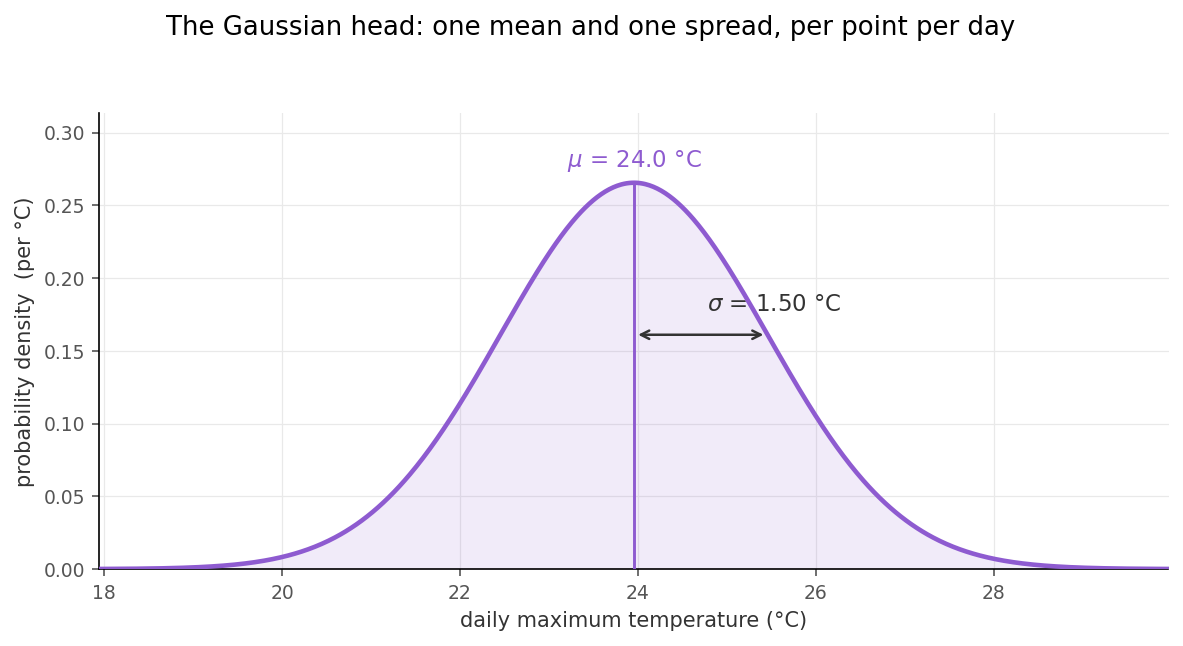
\includegraphics[width=0.9\textwidth]{images/16_tmax_distribution.png}
\caption[The Gaussian predictive distribution]{The Gaussian predictive density for a single target point and day. The model outputs the two parameters: the mean $\mu$ locates the distribution and the standard deviation $\sigma$ sets its width, shown here for $\mu = 24.0\,^{\circ}\mathrm{C}$ and $\sigma = 1.5\,^{\circ}\mathrm{C}$.}
\label{fig:meth-tmax-dist}
\end{figure}

\begin{figure}[H]
\centering
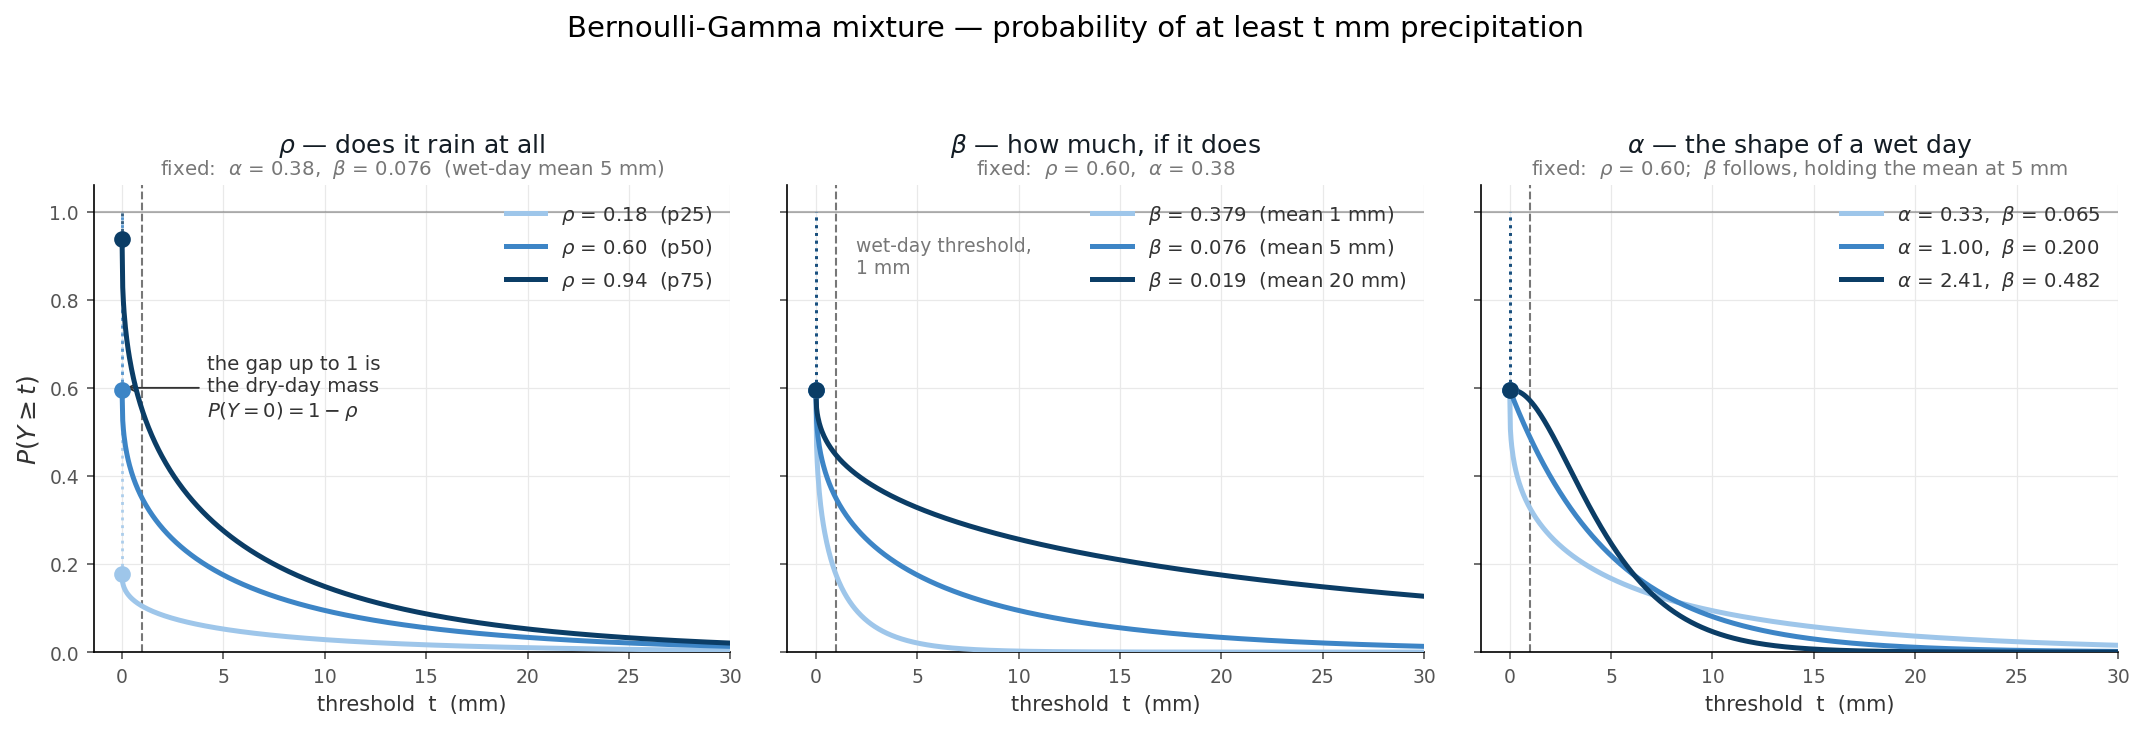
\includegraphics[width=\textwidth]{images/17_precip_wet_dry_day.png}
\caption[Bernoulli--Gamma distribution]{The Bernoulli--Gamma head read as the probability of at least $t$ millimetres, with one parameter turned per panel and the other two held constant. All parameter values are sampled from one of the model own outputs}
\label{fig:meth-precip-dials}
\end{figure}

\FloatBarrier
\section{Computational Cost}\label{sec:app-cost}

\sref{sec:meth-cost} gives the headline hardware requirement. The elevation MLP is where the cost
accumulates: it runs once per target point and never sees the input grid, and it accounts for most
of the arithmetic on both grids (\fref{fig:meth-cost-ops}). Underneath it the distance matrix holds
a fixed allocation that is far larger on the surface grid than on the atmospheric one, which is why
the atmospheric configuration is the cheaper of the two in memory as well as in operations despite
carrying many more input channels (\fref{fig:meth-cost-ops}, \fref{fig:meth-cost-mem}).

\begin{figure}[H]
    \centering
    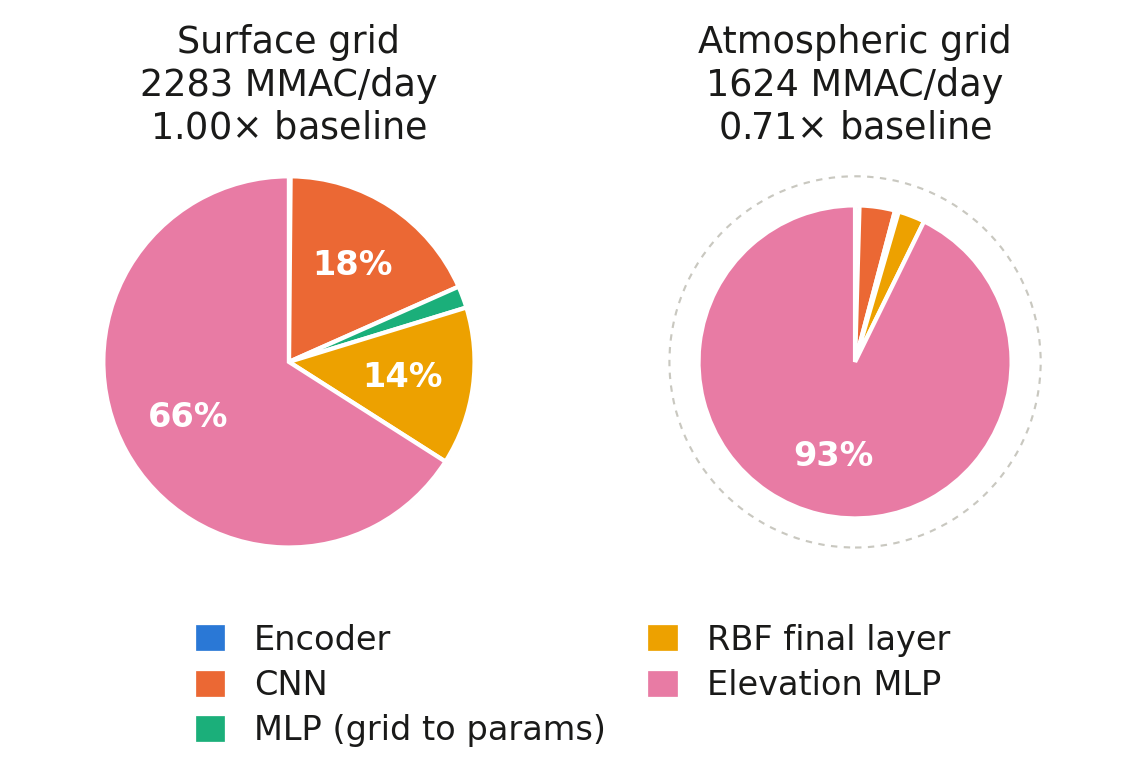
\includegraphics[width=0.75\textwidth]{images/component_cost_ops.png}
    \caption[Computational cost per component]{Computational cost per component: multiply-accumulate operations of one day, in millions, split into the architectural components.}
    \label{fig:meth-cost-ops}
\end{figure}

\begin{figure}[H]
    \centering
    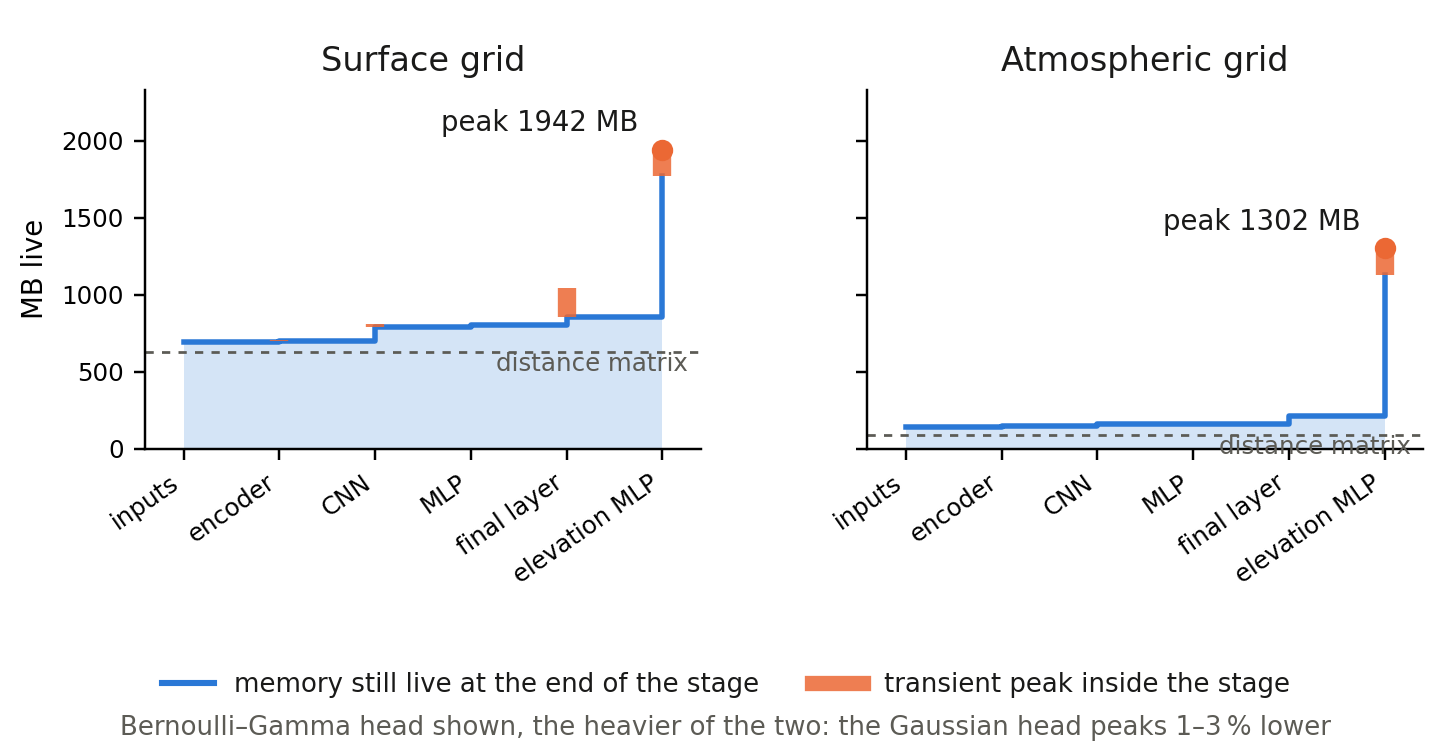
\includegraphics[width=0.86\textwidth]{images/component_cost_mem_profile.png}
    \caption[Memory through a training forward pass]{Memory estimation live at each stage of a training forward pass of the Bernoulli--Gamma configurations, the heavier of the two output heads, at the batch of eight days used in this work, with the transient inside each stage drawn above it. The peak is a moment inside a single stage, not a sum over stages.}
    \label{fig:meth-cost-mem}
\end{figure}

\FloatBarrier
\section{Additional Metric Definitions}\label{sec:app-metrics}

The metrics reported in this work are summarised in \tref{tab:meth-metrics-summary} and given in
full in \tref{tab:app-metrics-overview} below. Their definitions follow, together with the
properties of each that matter for reading \cref{ch:single-model}.

{\footnotesize
\begin{longtable}{|>{\raggedright\arraybackslash}p{3.1cm}|>{\raggedright\arraybackslash}p{0.6cm}|>{\raggedright\arraybackslash}p{3.3cm}|>{\raggedright\arraybackslash}p{6.3cm}|}
    \caption[Evaluation metrics in full]{Every metric \emph{reported} in this work, in full; \tref{tab:meth-metrics-summary} gives the short form.  Var: \textbf{T}emperature, \textbf{P}recipitation, or both. Range gives the theoretically possible values and the optimal direction.}
    \label{tab:app-metrics-overview} \\
    \hline
    \textbf{Metric} & \textbf{Var} & \textbf{Range (best)} & \textbf{Significance and use} \\
    \hline
    \endfirsthead
    \multicolumn{4}{l}{\textit{Table \thetable\ -- continued from previous page}} \\
    \hline
    \textbf{Metric} & \textbf{Var} & \textbf{Range (best)} & \textbf{Significance and use} \\
    \hline
    \endhead
    \hline
    \multicolumn{4}{r}{\textit{continued on next page}} \\
    \endfoot
    \hline
    \endlastfoot
        \multicolumn{4}{|l|}{\textit{Deterministic --- score the central prediction only}} \\
        \hline
        MAE (mean absolute error) & T, P & $[0,\infty)$, lower; in the variable's unit ($^{\circ}\mathrm{C}$ or $\mathrm{mm}$) & Headline error against the fixed truth; comparable across every run \\
        \hline
        RMSE (root-mean-square error) & T & $[0,\infty)\,^{\circ}\mathrm{C}$, lower & Same comparison, weighted towards large errors \\
        \hline
        Bias & T & $(-\infty,\infty)\,^{\circ}\mathrm{C}$, ideal $0$ & Tests for a systematic offset, using $n_{\mathrm{eff}}$ (\eref{eq:neff}) \\
        \hline
        MAE skill & P & $(-\infty,1]$, higher; $1$ perfect, $0$ = no better than ERA5-Land, negative worse & Deterministic-error skill vs.\ ERA5-Land (\eref{eq:mae-skill}); the one skill score built from a deterministic error rather than a proper score \\
        \hline
        Spearman $r_{S}$ (pooled) & P & $[-1,1]$, higher & Rank correlation between the predicted mean and the observation over the pooled point-days, subsampled to two million pairs with a fixed seed.  \\
        \hline
        \multicolumn{4}{|l|}{\textit{Probabilistic --- score the whole predictive distribution}} \\
        \hline
        CRPS (continuous ranked probability score) & T, P & $[0,\infty)$, lower; in the variable's unit ($^{\circ}\mathrm{C}$ or $\mathrm{mm}$) & The central proper score (\eref{eq:crps}) and the backbone of CRPSS below \\
        \hline
        CRPSS (CRPS skill score) & T & $(-\infty,1]$, higher; $1$ perfect, $0$ = baseline & CRPS-based skill vs.\ the bilinear input (\eref{eq:crpss}); comparable whenever the reference is shared\\
        \hline
        BSS (Brier skill score) & P & $(-\infty,1]$, higher; $1$ perfect, $0$ = baseline & Event skill: how much better the predicted probability of the binary event ``accumulation $\geq t$'' is than ERA5-Land's, at one threshold $t$ at a time (\eref{eq:bss}) \\
        \hline
        RPSS (ranked probability skill score) & P & $(-\infty,1]$, higher; $1$ perfect, $0$ = baseline & Whole-distribution categorical skill (\eref{eq:rpss}); penalises misplaced probability mass \\
        \hline
        R01 (wet-day frequency) & P & ratio, ideal $1$ & Predicted over observed fraction of days $\geq 1\,\mathrm{mm}$; the model's fraction is the analytic $P(Y \geq 1\,\mathrm{mm})$ of \eref{eq:bg-exceedance} evaluated at every target point and day, then averaged over them \\
        \hline
        Dry-day fraction & P & $[0,1]$, ideal $=$ observed & Fraction of days below $0.1\,\mathrm{mm}$; the model's value is $1 - P(Y \geq 0.1\,\mathrm{mm})$ evaluated at every target point and day, then averaged over them \\
        \hline
        SDII (simple daily intensity index) & P & $[0,\infty)\,\mathrm{mm}$, ideal $=$ observed & Mean accumulation on wet days. The model's value is the \emph{pooled} analytic wet-day intensity, $\sum \mathbb{E}[Y\,\mathbf{1}\{Y \geq 1\,\mathrm{mm}\}] \big/ \sum P(Y \geq 1\,\mathrm{mm})$ over all point-days \\
        \hline
        R10 & P & $[0,1]$, ideal $=$ observed & Fraction of days with accumulation $>10\,\mathrm{mm}$, strictly greater for the observations and the model alike. The model's value is the fraction of draws sampled from the predictive distribution that exceed $10\,\mathrm{mm}$, pooled over every target point and day \\
        \hline
        P98 & P & $[0,\infty)\,\mathrm{mm}$, ideal $=$ observed & 98th percentile of wet-day accumulation. The model's value is one percentile of the \emph{pooled} cloud of wet draws over all target points and days, not an average of per-point-day percentiles \\
        \hline
        PIT (probability integral transform) & T, P& Mean $[0,1]$, ideal $0.5$;\newline SD $[0,0.5]$, ideal $1/\sqrt{12}\approx0.289$ & Calibration diagnostic: whether the predicted quantiles are correct, read from a PIT histogram or Q--Q plot against the uniform. \\
        \hline
        Standardised-error SD & T & $[0,\infty)$, ideal $1$;\newline $<1$ forecast over-dispersed (predicted spread too wide),\newline $>1$ over-confident & Calibration diagnostic: whether the predicted spread matches the actual error spread \\
        \hline
        Coverage ($50\,\%$, $90\,\%$) & T & $[0,1]$,\newline ideal $=$ nominal\newline ($0.50$/$0.90$) & Calibration diagnostic: fraction of observations inside the nominal central interval \\
        \hline
\end{longtable}
}

\begin{table}[htbp]
    \centering
    \caption[Aggregation levels]{Aggregation levels. Within a regime (\sref{subsec:meth-cv}), the same
    metric can be read at any of these levels; the level is stated wherever a number is quoted.}
    \label{tab:app-eval-regimes}
    \footnotesize
    \begin{tabular}{|p{3.0cm}|p{10.3cm}|}
        \hline
        Pooled & Every valid target point and day of the regime is flattened into one array and averaged in a single pass, giving the headline number. A ratio-valued score is pooled as a ratio of the two pooled averages, never as an average of ratios \\
        \hline
        Per target point & Pooled over days only, giving a map. Whether its domain mean returns the pooled number depends on the metric: it does for MAE and bias, which are linear in the point-days, as long as every point carries the same number of valid days; it does not for RMSE, because a mean of square roots is not the square root of a mean; and it does not for any ratio-valued score (CRPSS, BSS, RPSS, MAE skill, R01, SDII), whose pooled and per-point forms are different quantities. The map is therefore read for \emph{where}, and the pooled number quoted for \emph{how much} \\
        \hline
        Per day & Pooled over target points only, into one domain-mean value per day; the basis of the bias significance test and of the monthly curves in \cref{ch:single-model} \\
        \hline
        Per fold (CV holdout only) & The pooled metric broken out by the five separately trained folds; the resulting spread distinguishes a stable ranking from one that should not be read too literally (\sref{subsec:single-precip-headline} uses it this way) \\
        \hline
    \end{tabular}
\end{table}

\subsection{Deterministic Errors and the CRPS}\label{subsec:app-crps}

\paragraph*{Standard error of the bias.}
Whether a mean error differs from zero cannot be judged by pooling every point and every day: the field is smooth and successive days are linked by the weather, so a nominal sample size of tens of millions would make any offset significant. Each day is therefore collapsed to its domain mean first, and the remaining serial correlation is absorbed into the effective sample size
\begin{equation}
    n_{\mathrm{eff}} \;=\; T \, \frac{1 - r_{1}}{1 + r_{1}} ,
    \label{eq:neff}
\end{equation}
with $T$ the number of days and $r_1$ the lag-1 autocorrelation of the daily series~\cite{wilks2019statistical}. Confidence intervals and $t$ tests use $n_{\mathrm{eff}}$ in place of $T$, which widens the standard error of the mean by a factor set entirely by $r_1$,
\begin{equation}
    \mathrm{SE}_{\mathrm{adj}} \;=\; \frac{s}{\sqrt{n_{\mathrm{eff}}}}
    \;=\; \frac{s}{\sqrt{T}} \sqrt{\frac{1 + r_1}{1 - r_1}}
    \;=\; \mathrm{SE} \, \sqrt{\frac{1 + r_1}{1 - r_1}} ,
    \label{eq:se-adj}
\end{equation}
where $s$ is the standard deviation of the daily means. Persistence is therefore paid for directly in interval width, and an offset has to clear a correspondingly higher bar before it counts as real: at $r_1 = 0.6$ the interval doubles, and at the autocorrelation of the 2024 holdout, which leaves about $220$ of its $366$ days effectively independent (\sref{subsec:single-tmax-discussion}), it widens by roughly $30\,\%$. This stops trivial noise from being labelled statistically significant merely because the pooled sample is large. The correction covers day-to-day persistence but not seasonal structure, so its intervals stay mildly optimistic. The daily series, $r_1$, $n_{\mathrm{eff}}$ and the resulting interval are produced by \texttt{scripts/gen\_bias\_significance.py} from the cached predictions of the regime being scored, one JSON per model and regime.

\paragraph*{Continuous ranked probability score (CRPS).}
The central probabilistic score is the continuous ranked probability score (CRPS)~\cite{gneiting2007scoring}, for a predictive CDF $F$ and an observation $y$
\begin{equation}
    \mathrm{CRPS}(F, y) \;=\; \int_{-\infty}^{\infty} \bigl( F(z) - \mathbf{1}\{z \geq y\} \bigr)^{2} \,\mathrm{d}z ,
    \label{eq:crps}
\end{equation}
the squared distance between the predicted CDF and the step function of the observation, strictly proper so that it rewards distributions that are both sharp and calibrated. It is closed-form for the Gaussian; for the Bernoulli--Gamma it is sample-estimated during training, while the station evaluation uses the closed form of the Gamma CRPS. For a deterministic forecast $x$ it collapses to $\lvert x - y \rvert$, so a probabilistic model and a deterministic baseline can be scored on one scale, which is the property every skill score below relies on.

\paragraph*{Probability integral transform (PIT).}
Calibration is assessed through the probability integral transform: if the predictive distributions are correct, the values $u = F(y)$ are uniform on $[0,1]$. The mixed distribution of precipitation needs one adjustment at its point mass (\sref{subsec:app-skill-precip}).

\subsection{Temperature Skill and Calibration}\label{subsec:app-skill-tmax}

\paragraph*{Skill against the interpolated input (CRPSS).}
The temperature reference forecast is the ERA5-Land daily maximum $2\,\mathrm{m}$ temperature field, $\mathrm{t2m\_max}$ on the $0.1^{\circ}$ grid of \tref{tab:data-grids}, bilinearly interpolated to the MeteoSwiss target points. This product is not the input grid of every model: the atmospheric configurations read ERA5 at $0.25^{\circ}$ and never see a surface field at all, so their reference is loaded separately rather than taken from their own context. Being deterministic, its CRPS equals its absolute error, and
\begin{equation}
    \mathrm{CRPSS} \;=\; 1 - \frac{\overline{\mathrm{CRPS}}_{\mathrm{model}}}{\overline{\mathrm{CRPS}}_{\mathrm{ref}}}
    \label{eq:crpss}
\end{equation}
is computed pooled and per target point, the map showing \emph{where} the model beats interpolation. Two runs are CRPSS-comparable only if they share the same reference construction: the same baseline file, the same target points and the same domain bounds. That condition is weaker than sharing an input grid, and satisfying it makes the comparison in \cref{ch:single-model} legitimate. Every temperature configuration in this work, surface and atmospheric alike, is scored against one and the same interpolated ERA5-Land field, so its CRPSS values differ from each other only through the numerator.

\paragraph*{Calibration of the Gaussian head.}
The PIT of \sref{subsec:app-crps} applies unchanged to the Gaussian. Two further diagnostics of \tref{tab:app-metrics-overview} are defined here rather than there because they are available for temperature only: both need a predicted mean and a predicted spread, and the Bernoulli--Gamma head of \sref{subsec:meth-likelihoods} carries neither as a parameter, so precipitation calibration rests on the PIT alone. The first standardises every error by the spread predicted at that point and day, $z = (y - \mu)/\sigma$. If the predicted spread is right, $z$ has a standard deviation of one; a value below one means the model predicts wider intervals than its errors require, a value above one that it is over-confident. The second is the central coverage: the fraction of observations falling inside the nominal $50\,\%$ and $90\,\%$ interval of the predictive distribution, read off the PIT values as the fraction landing in $[0.25, 0.75]$ and $[0.05, 0.95]$. Both are pooled over every valid target point and day of the regime, and both are reported alongside the PIT moments in the calibration figures of \cref{ch:single-model}.

\subsection{Precipitation Indices and Event-Based Skills}\label{subsec:app-skill-precip}

\paragraph*{Physical indices instead of squared error.}
Squared-error measures summarise daily precipitation poorly: the field is zero on most days and heavily skewed on wet days, while what matters is occurrence, intensity and extremes. Following \textcite{vaughan2022convcnp}, the precipitation models are judged on the physical indices of \tref{tab:app-metrics-overview}. No wet/dry classification with a fixed probability cut is ever applied. Wherever an occurrence statistic can be, it is instead read from the exceedance probability of \eref{eq:bg-exceedance}, evaluated at the threshold that statistic is defined by: $1\,\mathrm{mm}$ for the wet-day frequency and R01, $0.1\,\mathrm{mm}$ for the dry-day fraction, and each of the four thresholds of the Brier skill maps below. Note that these are two different cuts and are kept apart throughout: $1\,\mathrm{mm}$ is the wet-day definition this chapter and its indices are built on, while $0.1\,\mathrm{mm}$ is the any-rain cut separating a dry day from drizzle. The next paragraph gives the route taken by the indices that have no such closed form.

\paragraph*{From point-day distributions to pooled frequencies.}
\fref{fig:meth-precip-dials} reads the distribution at a single point and day, whereas the results report \emph{frequencies} pooled over many points and days. Two routes turn one into the other. Where the quantity has a closed form in $(\rho, \alpha, \beta)$, the per-point-day probability \emph{is} that day's contribution to the event's rate, so averaging it gives the frequency exactly; this is how R01 and the wet-day-frequency maps are read off. Where no closed form exists, as for R10, P98 and the intensity categories, the model is sampled at each point and day and the frequency or percentile computed from those draws as it would be from observations.

\paragraph*{PIT at the point mass.}
The probability integral transform of \sref{subsec:app-crps} needs one adjustment for a distribution that puts finite probability on the single value zero. It takes the standard randomisation at that point mass, drawing $u$ uniformly from $[0, 1-\rho]$ whenever the observed day is dry ($y \leq 0.05\,\mathrm{mm}$), so that a correct model still returns uniform values.

\paragraph*{Brier skill score (BSS).}
The precipitation skill scores are event-based~\cite{wilks2019statistical} against the ERA5-Land total precipitation field, bilinearly interpolated and treated as a deterministic forecast. All three of them, the Brier skill here, the MAE skill and the RPSS below, are scored against a reference re-accumulated over the same $06$--$06\,\mathrm{UTC}$ window as RhiresD rather than over the UTC calendar day, so reference and target cover the same twenty-four hours. This is deliberately not the field the model reads: the input channel keeps the calendar-day total of \sref{subsec:data-coords}, and only the scoring reference is rebuilt on the target's window. The model issues $P(Y \geq t)$, scored by the Brier score $\mathrm{BS} = \overline{(p - o)^{2}}$ with $o \in \{0,1\}$ the observed event, giving
\begin{equation}
    \mathrm{BSS} \;=\; 1 - \frac{\mathrm{BS}_{\mathrm{model}}}{\mathrm{BS}_{\mathrm{ref}}}
    \label{eq:bss}
\end{equation}
mapped per target point at $t \in \{0.1, 10, 40, 80\}\,\mathrm{mm}$, from any-rain to the heavy tail. One property of the score has to be carried into any summary of the map. Where the reference never errs on the event, $\mathrm{BS}_{\mathrm{ref}} = 0$ and the ratio is undefined, so those target points are dropped rather than counted as a tie. They are the points the reference finds easiest, which means a domain median or mean of the BSS map is taken over a subset from which the reference's best-served locations have been removed.

\paragraph*{MAE skill.}
Since MAE is reported for every run, it can be scored against the same reference,
\begin{equation}
    \mathrm{MAE\text{-}skill} \;=\; 1 - \frac{\mathrm{MAE}_{\mathrm{model}}}{\mathrm{MAE}_{\mathrm{ref}}} ,
    \label{eq:mae-skill}
\end{equation}
which unlike BSS and RPSS scores only the central prediction, a difference that matters since \sref{subsec:single-precip-headline} finds it disagrees in sign with RPSS.

That disagreement is not an accident of the data, and the definition of the central prediction is where it starts. The point forecast entering both the MAE and the rank correlation is the mixture mean $\mathbb{E}[Y] = \rho\,\alpha/\beta$, the like-for-like counterpart of the single value the deterministic reference issues. But the absolute error is minimised by the \emph{median}, not the mean, and for a distribution with most of its mass at zero the two are far apart: a model that honestly reports a $40\,\%$ chance of $8\,\mathrm{mm}$ returns a mean of about $3\,\mathrm{mm}$ on a day that will most likely stay dry. Reporting the median instead would lower every run's MAE, but it would also throw away the amount the model is least sure about, and it would no longer be the quantity the reference is compared against. The mean is kept, and the resulting penalty is understood as the price a distribution pays when it is scored by a metric that rewards the safest single number.

\paragraph*{Ranked probability skill score (RPSS).}
To judge the intensity structure as a whole, the accumulation is divided into the ordered categories $[0, 0.1)$, $[0.1, 10)$, $[10, 40)$, $[40, 80)$ and $[80, \infty)\,\mathrm{mm}$ and scored with the ranked probability score, the squared distance between the forecast and observed CDFs accumulated over the internal boundaries $t_k$:
\begin{equation}
    \mathrm{RPS} \;=\; \sum_{k} \bigl( F(t_k) - \mathbf{1}\{y < t_k\} \bigr)^{2},
    \qquad
    \mathrm{RPSS} \;=\; 1 - \frac{\overline{\mathrm{RPS}}_{\mathrm{model}}}{\overline{\mathrm{RPS}}_{\mathrm{ref}}} .
    \label{eq:rpss}
\end{equation}
Both are reported per target point and pooled over the domain.
\FloatBarrier
\section{Temperature Model Metrics}\label{sec:app-tmax-metrics}

The headline metrics of the seven temperature runs are given in \tref{tab:single-tmax-headline} of \cref{ch:single-model}; the figures below support them.


\begin{figure}[H]
\centering
\subfloat[against target altitude]{%
  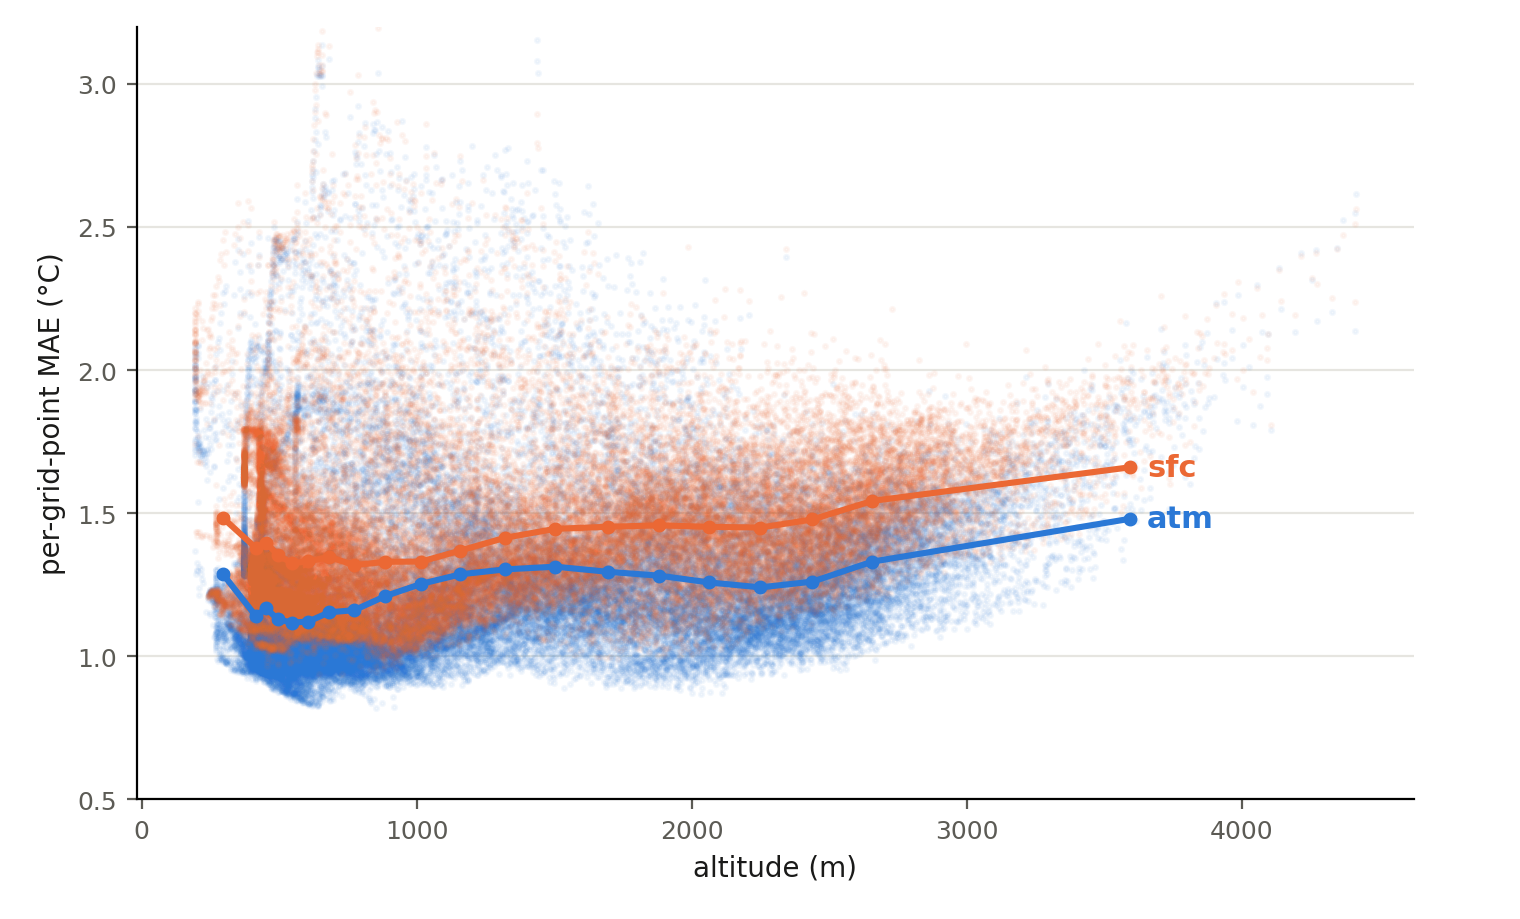
\includegraphics[width=0.49\textwidth]{images/tmax_mae_vs_altitude_overlay_cv.png}}
\hfill
\subfloat[against elevation mismatch, logarithmic axis]{%
  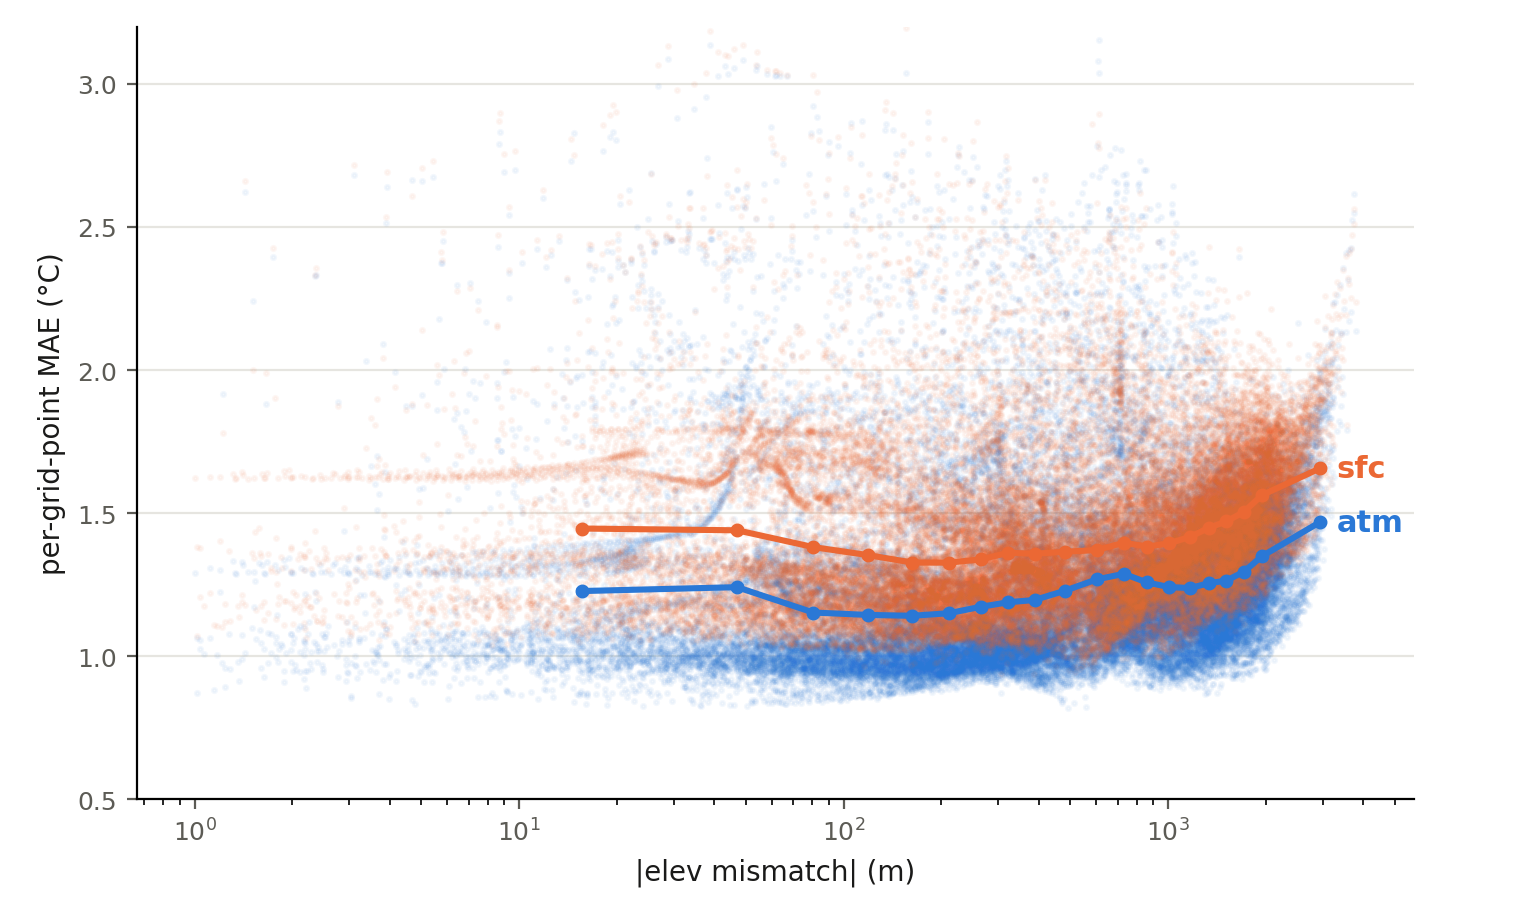
\includegraphics[width=0.49\textwidth]{images/tmax_mae_vs_elevmismatch_overlay_cv.png}}
\caption[Per-pixel error against altitude and against elevation mismatch]{Per-grid-point MAE over the CV holdout against altitude and against elevation mismatch, for \texttt{sfc} and \texttt{atm} (\sref{subsec:single-tmax-geography}). Every grid point is plotted; the heavy line is the binned median. The panels differ only in the horizontal variable.}
\label{fig:single-tmax-terrain}
\end{figure}

\begin{figure}[H]
\centering
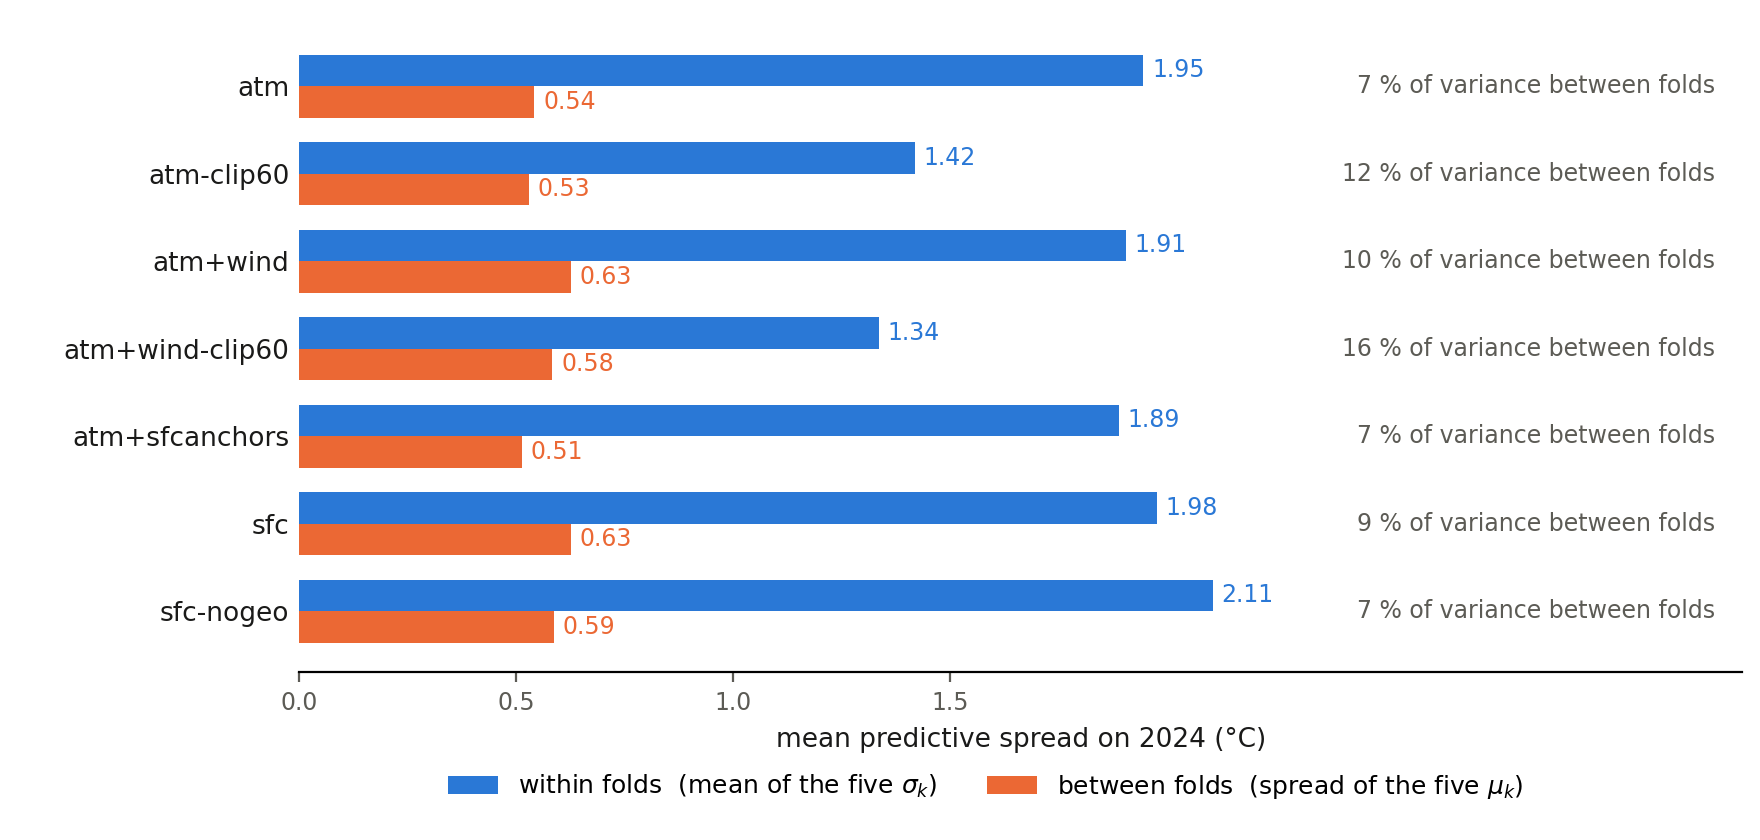
\includegraphics[width=0.9\textwidth]{images/tmax_sigma_decomposition.png}
\caption[Decomposition of the 2024 predictive spread, all models]{Decomposition of the mean 2024 predictive spread into its two moment-matching parts for all seven temperature models: the mean single-fold spread and the disagreement of the five fold means. The selected model \texttt{atm+wind-clip60} carries the largest between-fold variance of $16\,\%$ }
\label{fig:app-sigma-decomposition}
\end{figure}

\begin{figure}[H]
\centering
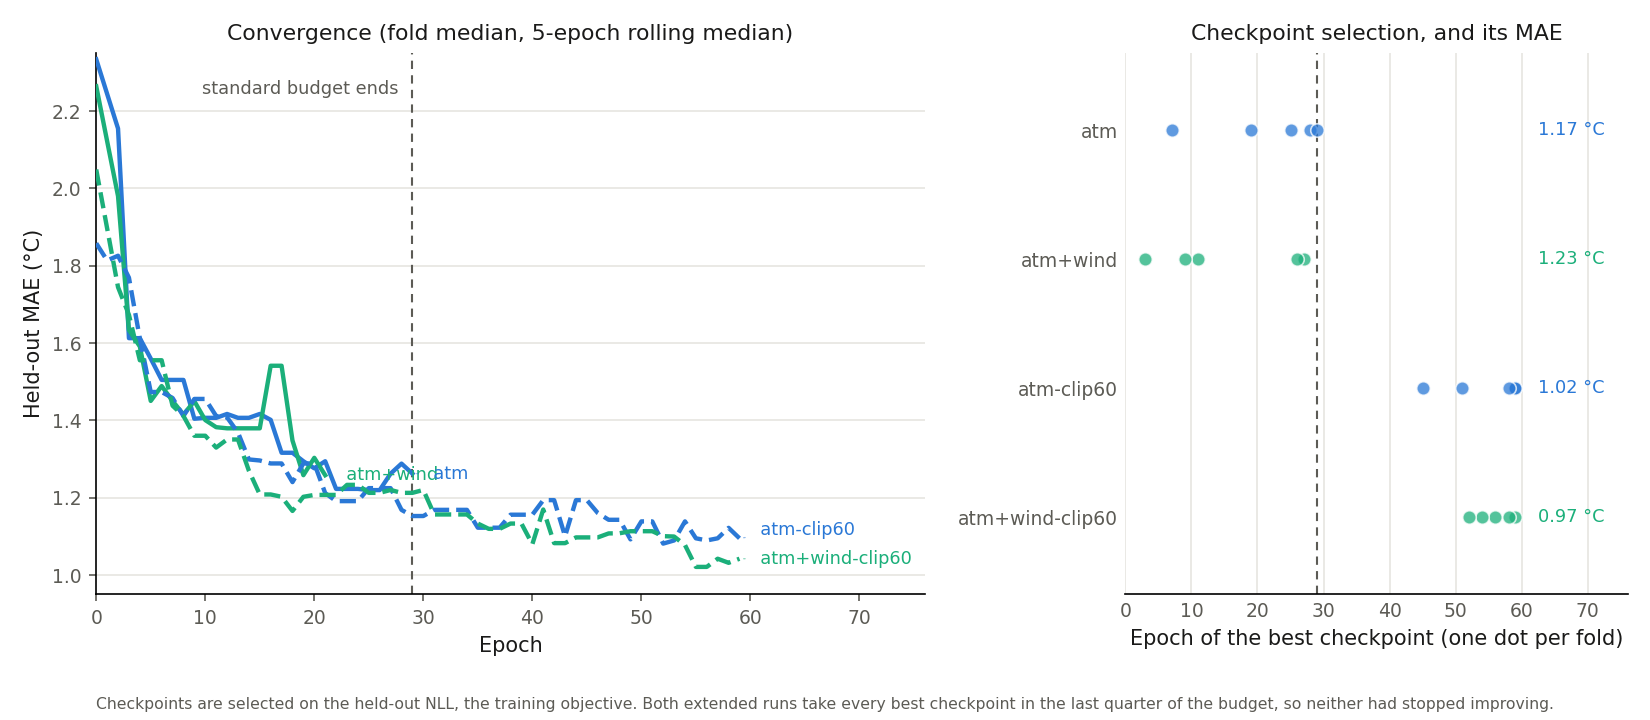
\includegraphics[width=\textwidth]{images/tmax_convergence_wind.png}
\caption[Convergence of the wind ablation under both training budgets]{Convergence of the two
atmospheric configurations with and without the wind channels, under the standard and the extended
training budget. Left: the held-out score written at each epoch during training, as the median over
the five folds and smoothed with a five-epoch rolling median, since the epoch-to-epoch scatter is
larger than the difference between the runs. Right: the epoch at which each fold's best checkpoint
was taken, one dot per fold, with the median held-out MAE of those checkpoints beside it. Selection
is on the held-out negative log-likelihood, the training objective, so the right panel is the
quantity that actually decided which weights entered \cref{ch:single-model}. At the standard budget
the wind model is behind ($1.23$ against $1.17\,^{\circ}\mathrm{C}$) and three of its five folds stop
early; under the extended budget the order reverses ($0.97$ against $1.02$) and every one of its
best checkpoints falls between epochs $52$ and $59$, so it had not stopped improving when the run
ended. The curve is a median over days while the headline MAE of \tref{tab:single-tmax-headline} is
a mean over all point-days, so the levels here are not directly comparable with that table; the
ordering and the trend are.}
\label{fig:app-tmax-convergence}
\end{figure}

Under the standard budget three of the five \texttt{atm+wind} folds stop early, whereas under the
extended one every fold of \texttt{atm+wind-clip60} takes its best checkpoint between epochs $52$ and
$59$: the run was still improving when it ended, which is why the extra channels only pay off once the
budget is long enough to incorporate them (\sref{subsec:single-tmax-headline}).

\FloatBarrier
\section{Feature Importance}\label{sec:app-fi}

Every attribution reproduced here is scored on the 2024 holdout year, the regime of
\tref{tab:meth-fi-setup}, so the permutation and LIME results can be read against each other
directly. The section is arranged in two steps: the selected models in full, including their
per-channel resolution, then every configuration side by side in one figure per method.

\subsection{Selected Models}\label{subsec:app-fi-selected}

For each selected model the two methods are placed in one figure, permutation above and LIME below,
each grouped view followed by its per-channel counterpart.

\begin{figure}[p]
\centering
\subfloat[Grouped permutation importance]{%
  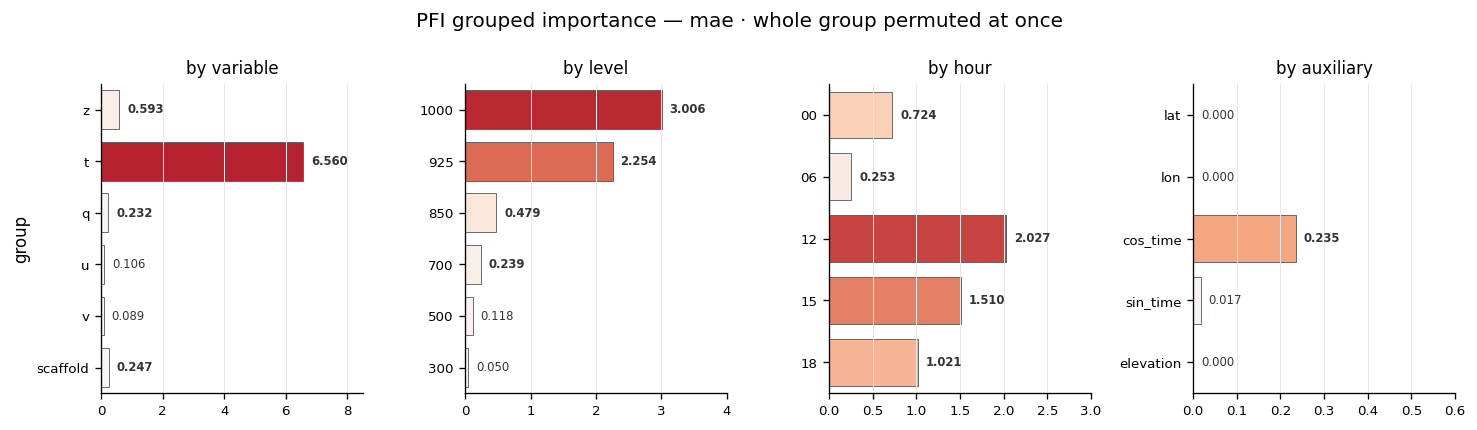
\includegraphics[width=0.84\textwidth,height=3.9cm,keepaspectratio]{images/results/tmax__pfi_groups_mae__feature_importance_2024__lbclip_wind.png}}\\[1ex]
\subfloat[Per-channel permutation importance]{%
  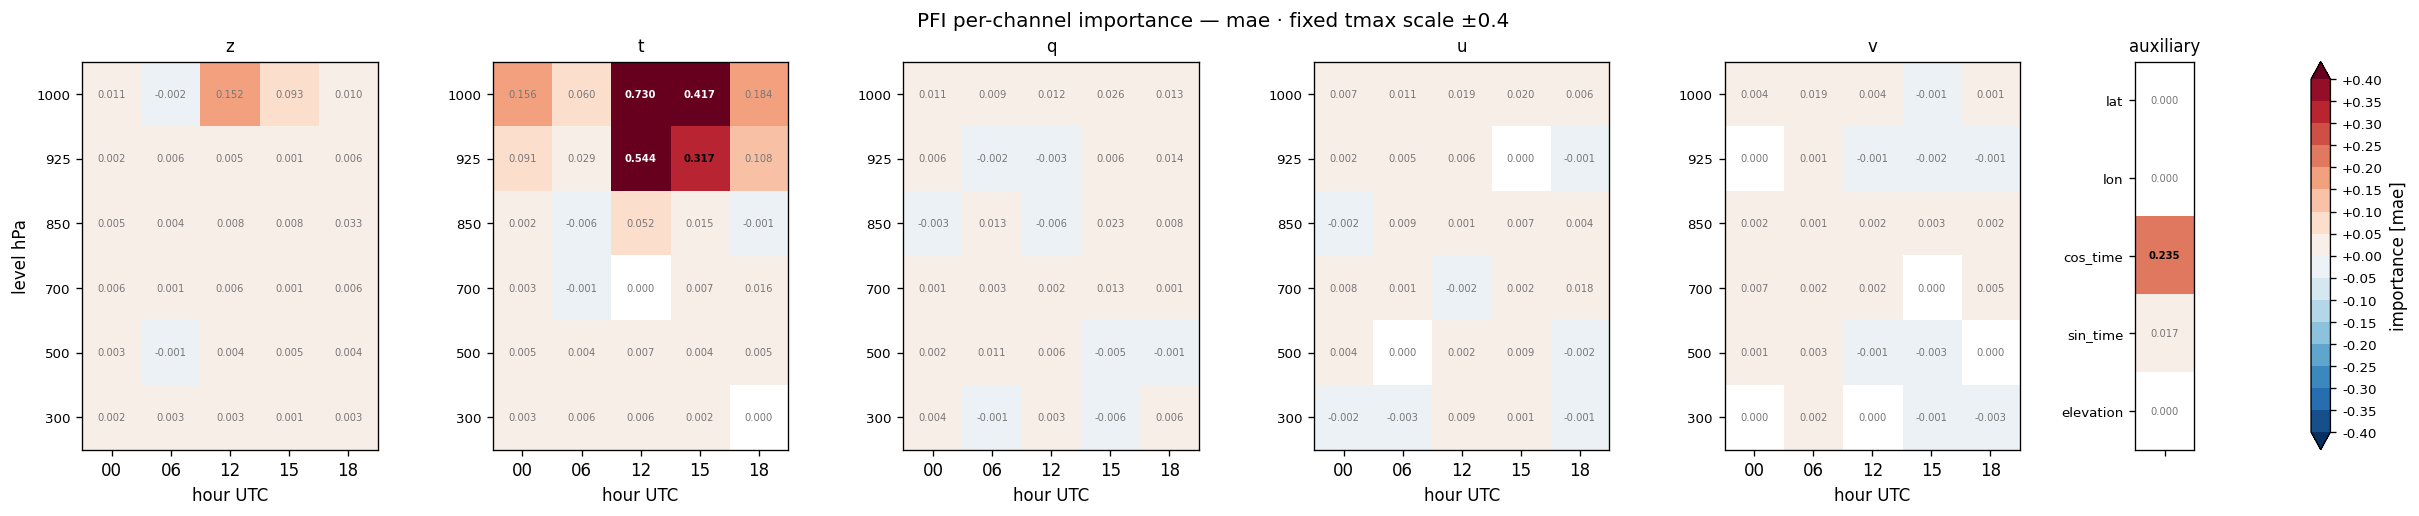
\includegraphics[width=0.84\textwidth,height=3.9cm,keepaspectratio]{images/results/tmax__pfi_heatmap_mae__feature_importance_2024__lbclip_wind.png}}\\[1ex]
\subfloat[Grouped LIME feature importance]{%
  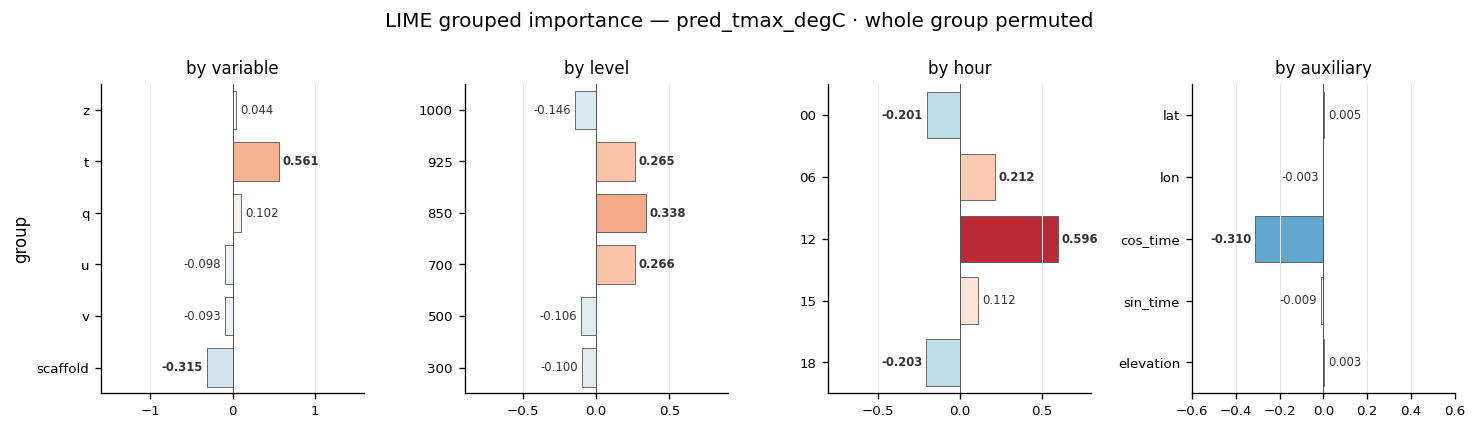
\includegraphics[width=0.84\textwidth,height=3.9cm,keepaspectratio]{images/results/tmax__lime_groups_pred_tmax_degC__feature_importance_2024__lbclip_wind.png}}\\[1ex]
\subfloat[Per-channel LIME feature importance]{%
  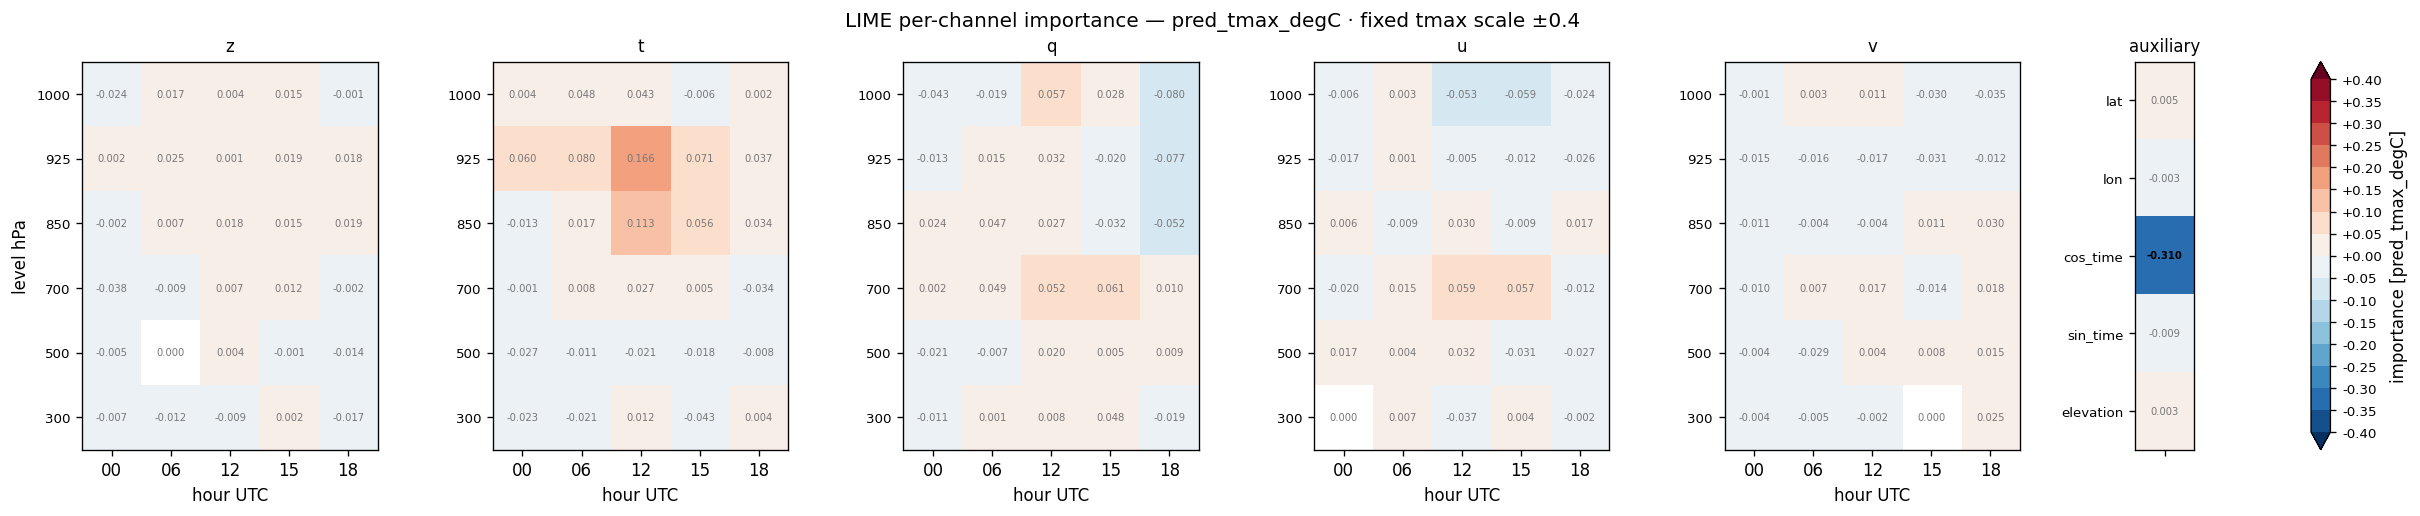
\includegraphics[width=0.84\textwidth,height=3.9cm,keepaspectratio]{images/results/tmax__lime_heatmap_pred_tmax_degC__feature_importance_2024__lbclip_wind.png}}
\caption[Feature Importance of the selected temperature model]{Feature Importance of the selected temperature model \texttt{atm+wind-clip60}. Permutation importance
is an MAE degradation in degrees Celsius, LIME a signed effect on the spatial-mean prediction in the
same unit, so the two panels of each pair share a unit but not a meaning. Temperature dominates the
grouped permutation view while the wind groups rank last among the meteorological variables, and the
level and hour patterns match the wind-free models, led by $1000$ and $925\,\mathrm{hPa}$ and the
midday hours. LIME agrees on those essentials: temperature leads, 12~UTC is the leading hour, and
the wind groups carry small coefficients. The per-channel panels are close to blank in the wind
groups at the shared scale, so no single wind channel carries visible importance on its own.}
\label{fig:app-fi-sel-tmax}
\end{figure}

\begin{figure}[p]
\centering
\subfloat[Grouped permutation importance]{%
  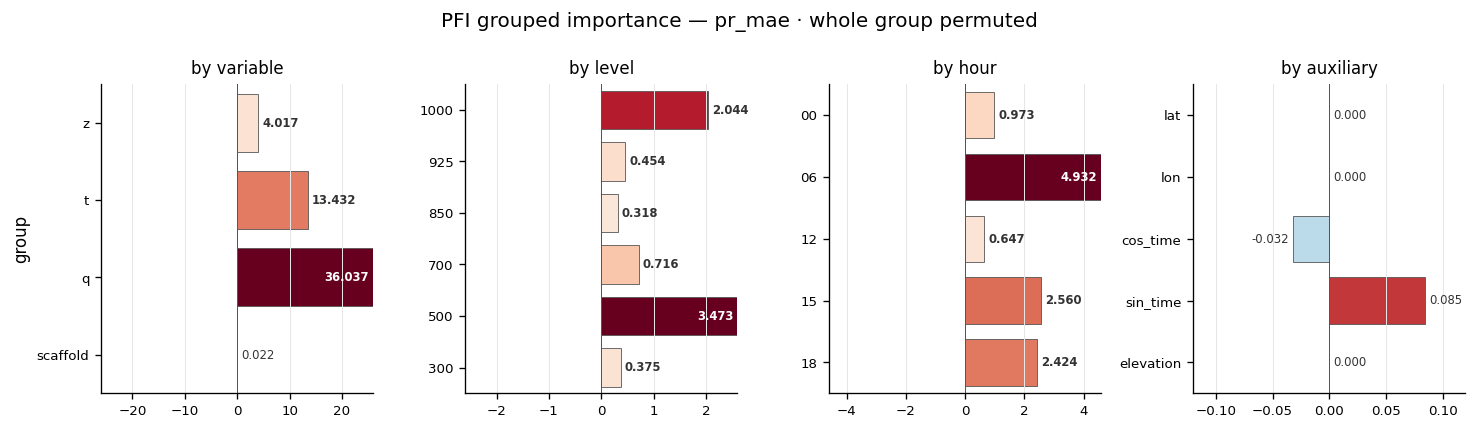
\includegraphics[width=0.84\textwidth,height=3.9cm,keepaspectratio]{images/results/precip__pfi_groups_pr_mae__feature_importance_2024__clean_solo_precip_ftcrps.png}}\\[1ex]
\subfloat[Per-channel permutation importance]{%
  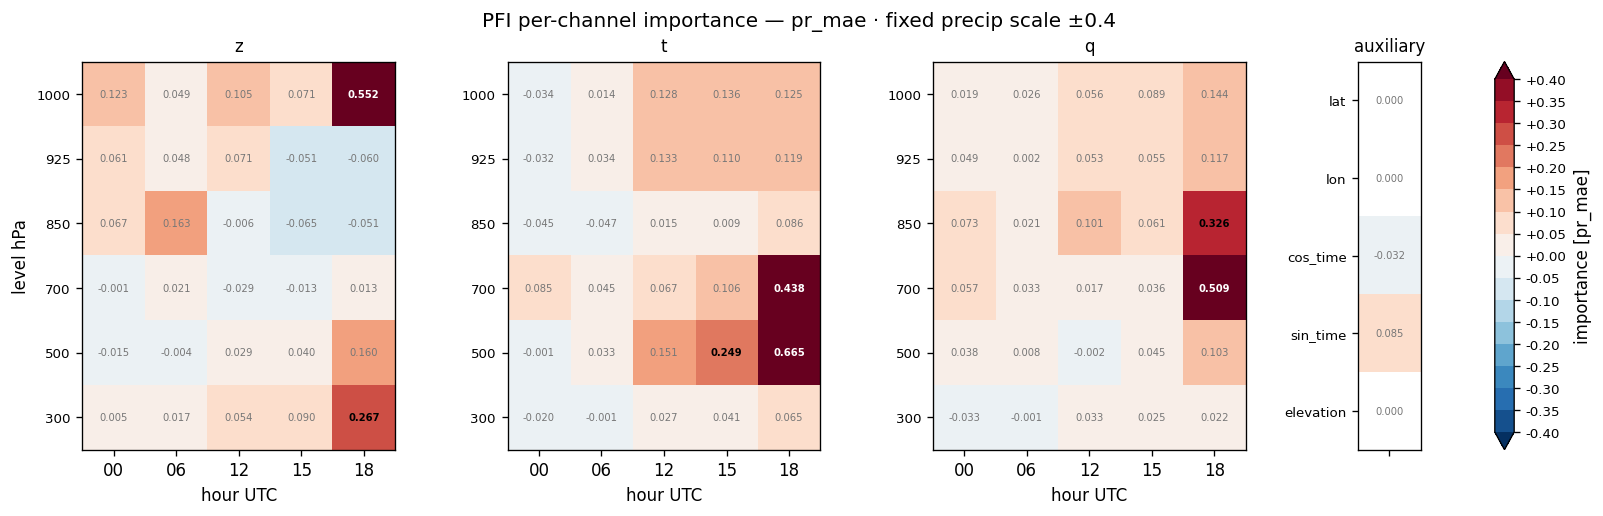
\includegraphics[width=0.84\textwidth,height=3.9cm,keepaspectratio]{images/results/precip__pfi_heatmap_pr_mae__feature_importance_2024__clean_solo_precip_ftcrps.png}}\\[1ex]
\subfloat[Grouped LIME feature importance]{%
  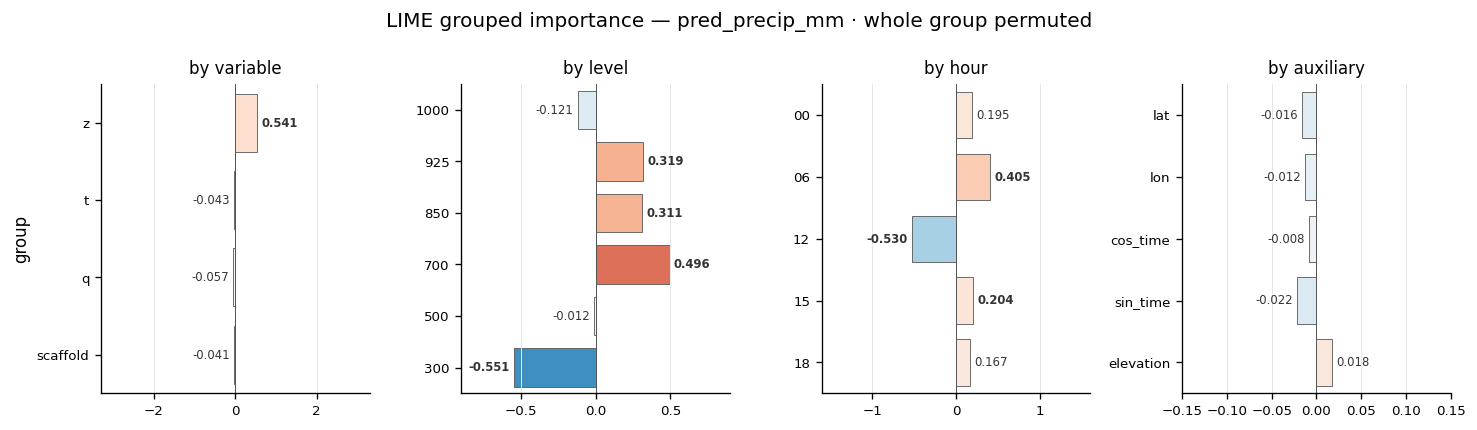
\includegraphics[width=0.84\textwidth,height=3.9cm,keepaspectratio]{images/results/precip__lime_groups_pred_precip_mm__feature_importance_2024__clean_solo_precip_ftcrps.png}}\\[1ex]
\subfloat[Per-channel LIME feature importance]{%
  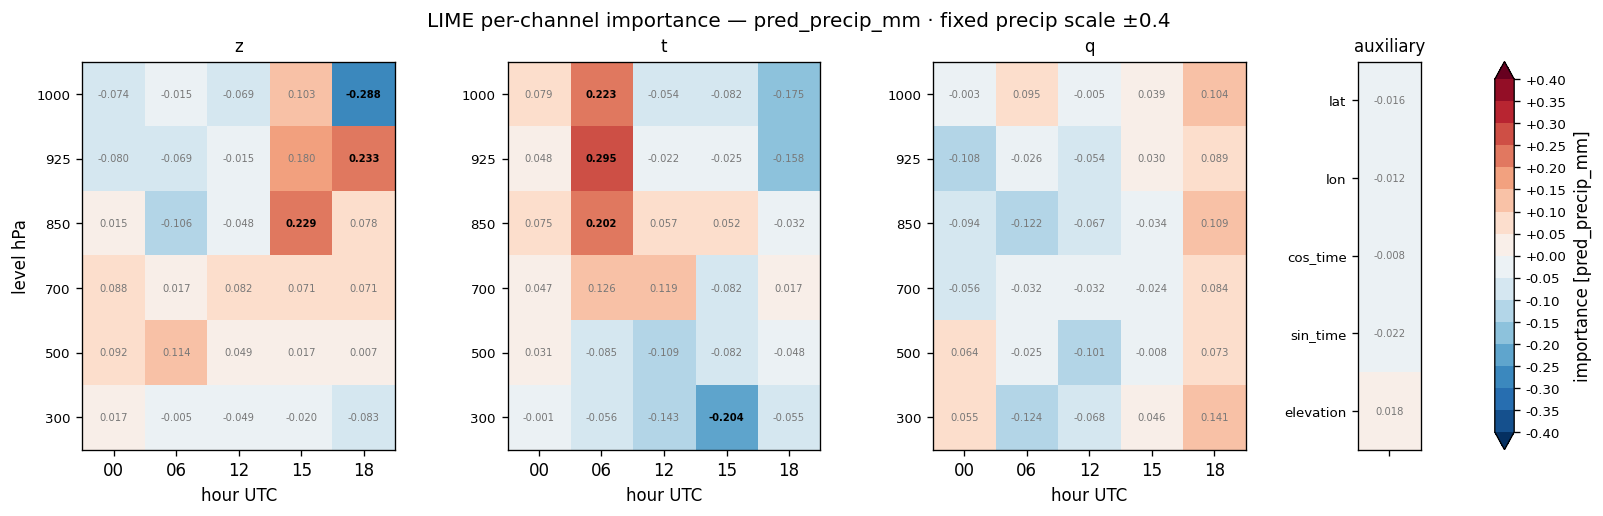
\includegraphics[width=0.84\textwidth,height=3.9cm,keepaspectratio]{images/results/precip__lime_heatmap_pred_precip_mm__feature_importance_2024__clean_solo_precip_ftcrps.png}}
\caption[Feature Importance of the selected atmospheric precipitation model]{Feature Importance of \texttt{precip-FT-CRPS}, the selected atmospheric precipitation model, in
millimetres. The grouped permutation view puts specific humidity far ahead of temperature and
geopotential and 06~UTC ahead of the other hours. LIME does not reproduce that ordering, which is
discussed in \sref{subsec:app-fi-lime}; for precipitation the permutation result is the one carried
forward.}
\label{fig:app-fi-sel-precip-ft}
\end{figure}

\begin{figure}[p]
\centering
% This model has seven channels and no levels or hours, so its panels are near-square
% rather than the 3:1 of the atmospheric runs: 2x2 uses the page, 4x1 does not.
\subfloat[Grouped permutation importance]{%
  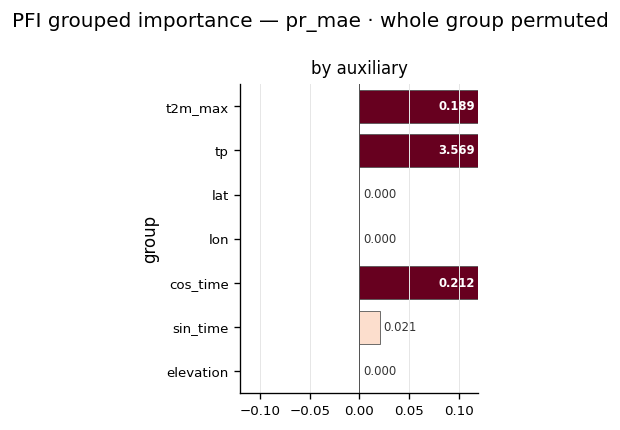
\includegraphics[width=0.47\textwidth,height=5.0cm,keepaspectratio]{images/results/precip__pfi_groups_pr_mae__feature_importance_2024__clean_solo_precip_sfctp.png}}\hfill
\subfloat[Grouped LIME feature importance]{%
  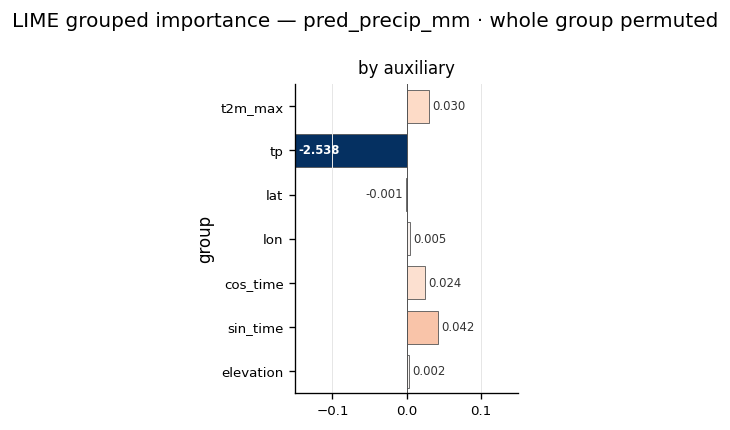
\includegraphics[width=0.47\textwidth,height=5.0cm,keepaspectratio]{images/results/precip__lime_groups_pred_precip_mm__feature_importance_2024__clean_solo_precip_sfctp.png}}\\[1ex]
\subfloat[Per-channel permutation importance]{%
  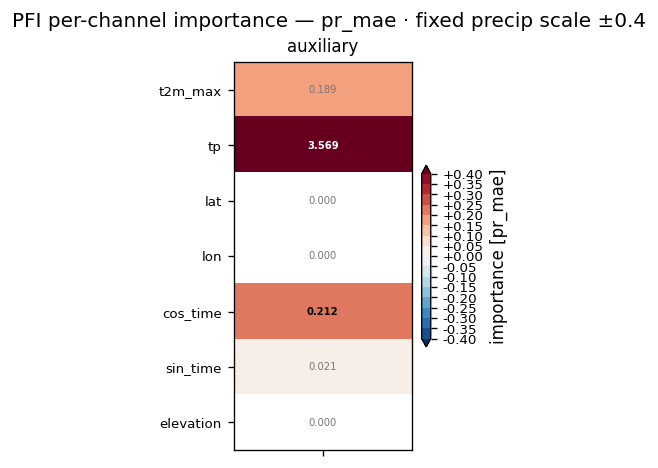
\includegraphics[width=0.47\textwidth,height=5.0cm,keepaspectratio]{images/results/precip__pfi_heatmap_pr_mae__feature_importance_2024__clean_solo_precip_sfctp.png}}\hfill
\subfloat[Per-channel LIME feature importance]{%
  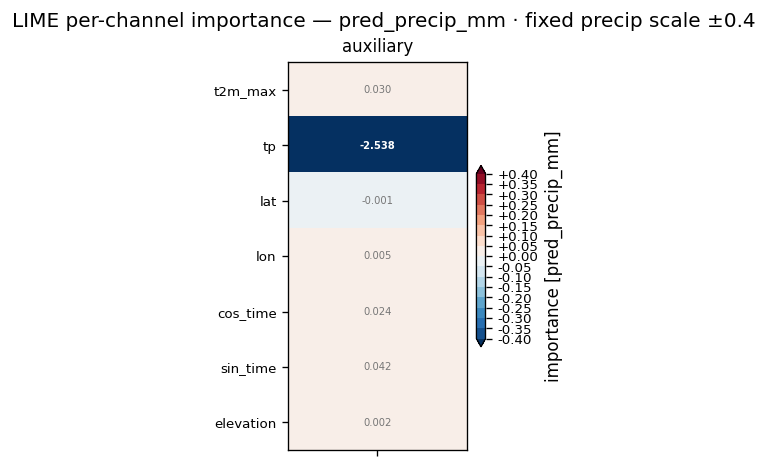
\includegraphics[width=0.47\textwidth,height=5.0cm,keepaspectratio]{images/results/precip__lime_heatmap_pred_precip_mm__feature_importance_2024__clean_solo_precip_sfctp.png}}
\caption[Feature Importance of the selected surface precipitation model]{Feature Importance of \texttt{precip-SFC-TP}, the selected surface precipitation model, in
millimetres. With no pressure levels or sampling hours to group by, the grouping collapses to the
seven channels themselves. Permutation gives the coarse \texttt{tp} accumulation almost the whole of
the model's importance; LIME gives the same channel a large negative coefficient, which is the
clearest illustration of the sign caveat in \sref{subsec:app-fi-lime}.}
\label{fig:app-fi-sel-precip-sfc}
\end{figure}

\FloatBarrier
\subsection{All Configurations at a Glance}\label{subsec:app-fi-allmodels}

Rather than one figure per configuration, every model of a variable is placed in a single figure per
method. One property of these figures has to be read before their bars: each bar is a \emph{share of
that model's largest group in the panel}, and the labelled bar carries the absolute value it was
scaled by. Bar lengths are therefore comparable \emph{within} a model and not between models, which
is the opposite convention to every other importance figure in this work. This normalisation is
required to make the comparison possible at all, since the surface models carry their whole importance in one
channel while the atmospheric models spread it over ninety or, with wind, a hundred and fifty.

The precipitation permutation view is not repeated here: it is
\fref{fig:single-precip-fi} in the main text.

\begin{figure}[h]
\centering
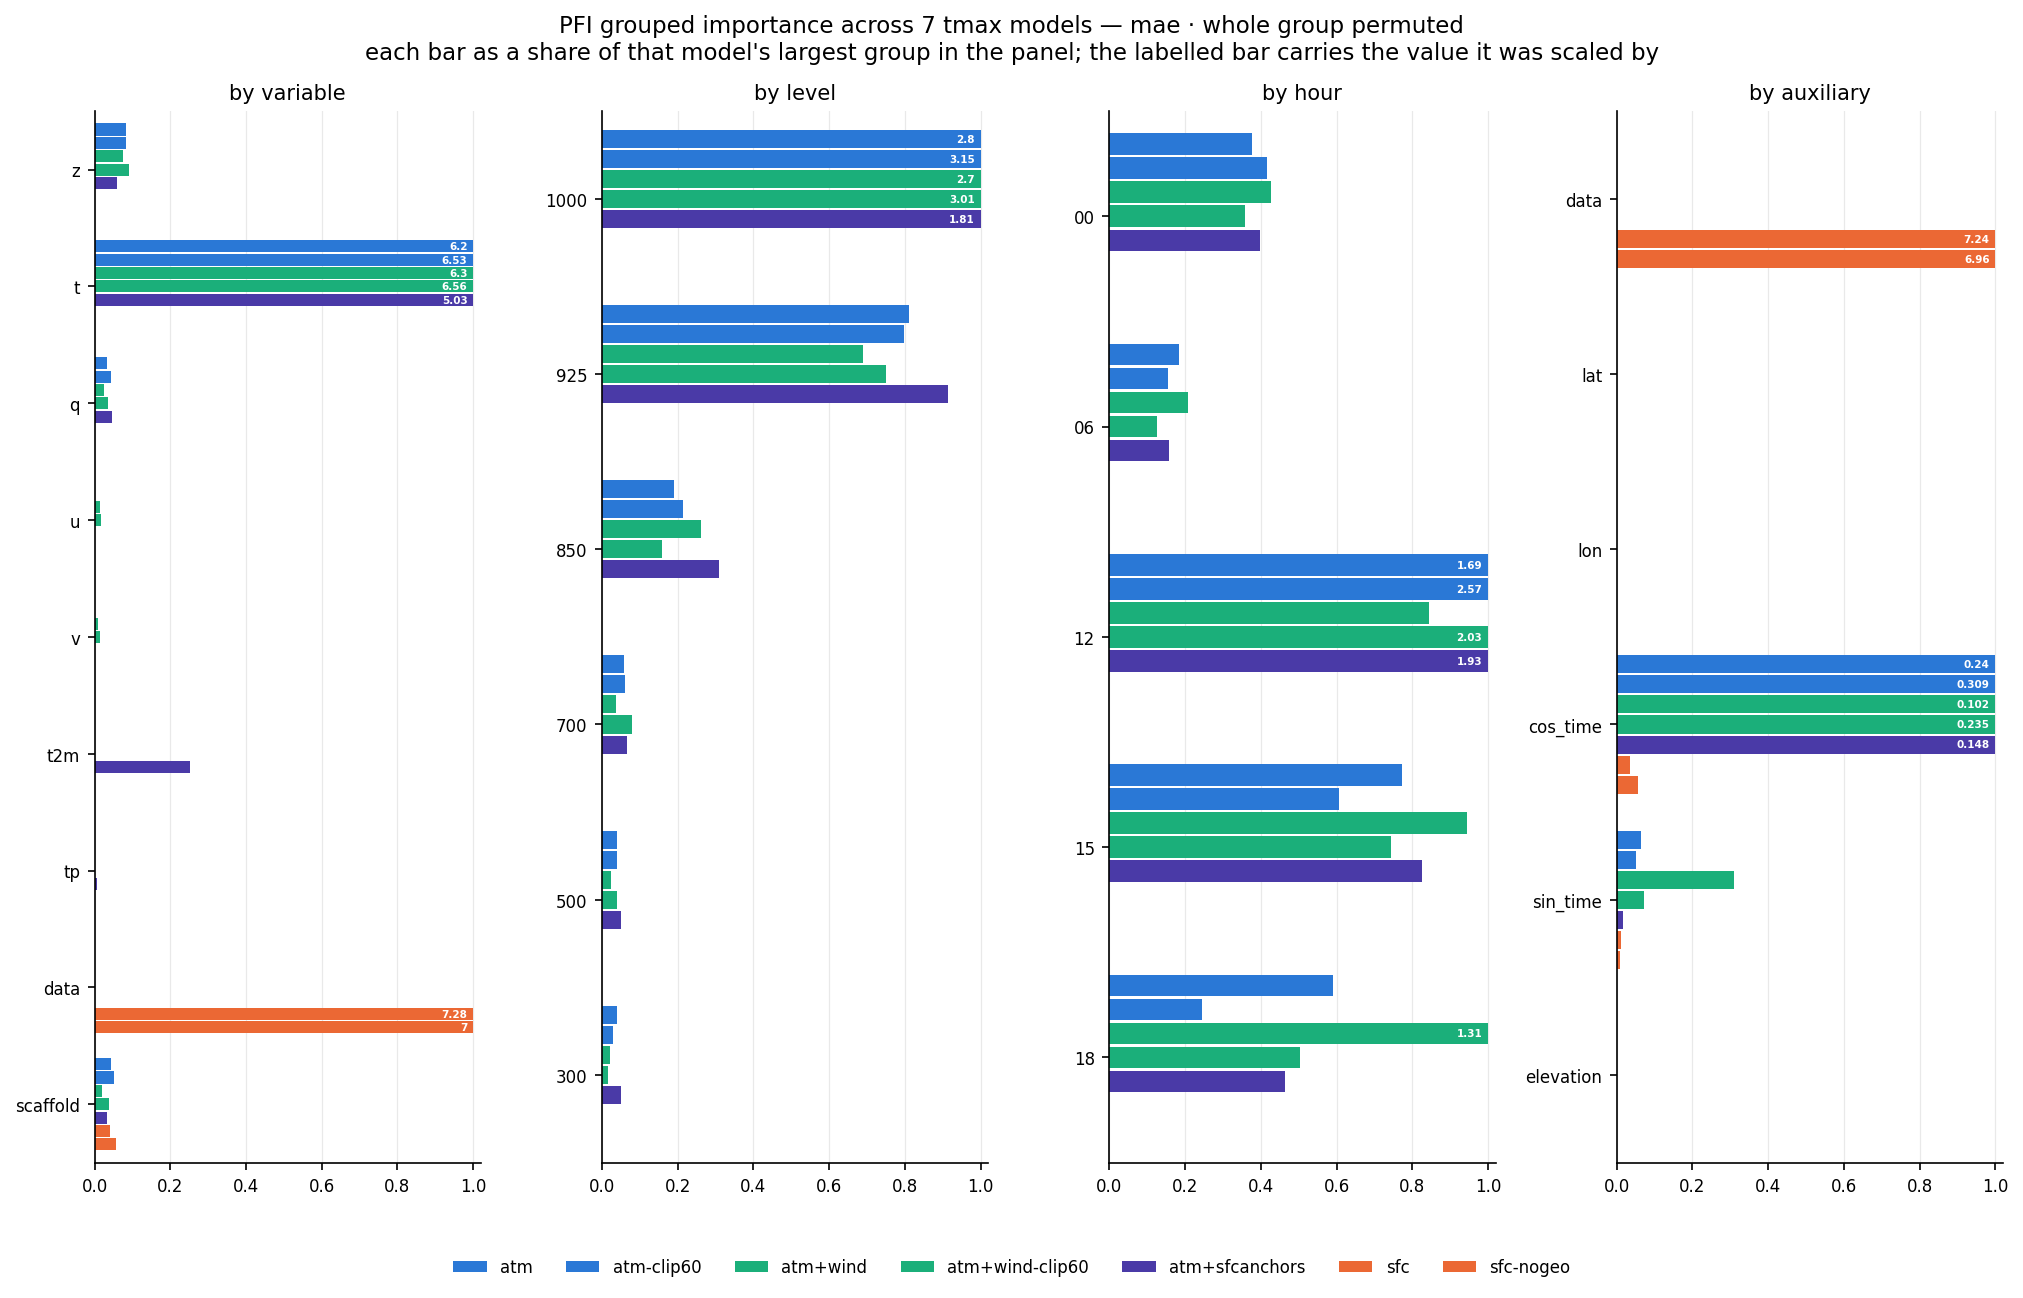
\includegraphics[width=\textwidth]{images/results/tmax__fi_group_importance_pfi_2024__tmax_model_comparison__ALL.png}
\caption[Grouped permutation importance across all temperature models]{Grouped permutation
importance of all seven temperature configurations, on the 2024 holdout. Each bar is a share of that
model's largest group in its panel and the labelled bars carry the degrees Celsius they were scaled
by, so the panels compare the \emph{shape} of a model's reliance rather than its magnitude. The two
surface models put everything into their single data channel; the five atmospheric ones agree on
temperature over geopotential and humidity, on $1000$ and $925\,\mathrm{hPa}$ over the levels above,
and on the midday and afternoon hours, with the wind groups $u$ and $v$ negligible in both runs that
carry them.}
\label{fig:app-fi-all-tmax-pfi}
\end{figure}

\begin{figure}[h]
\centering
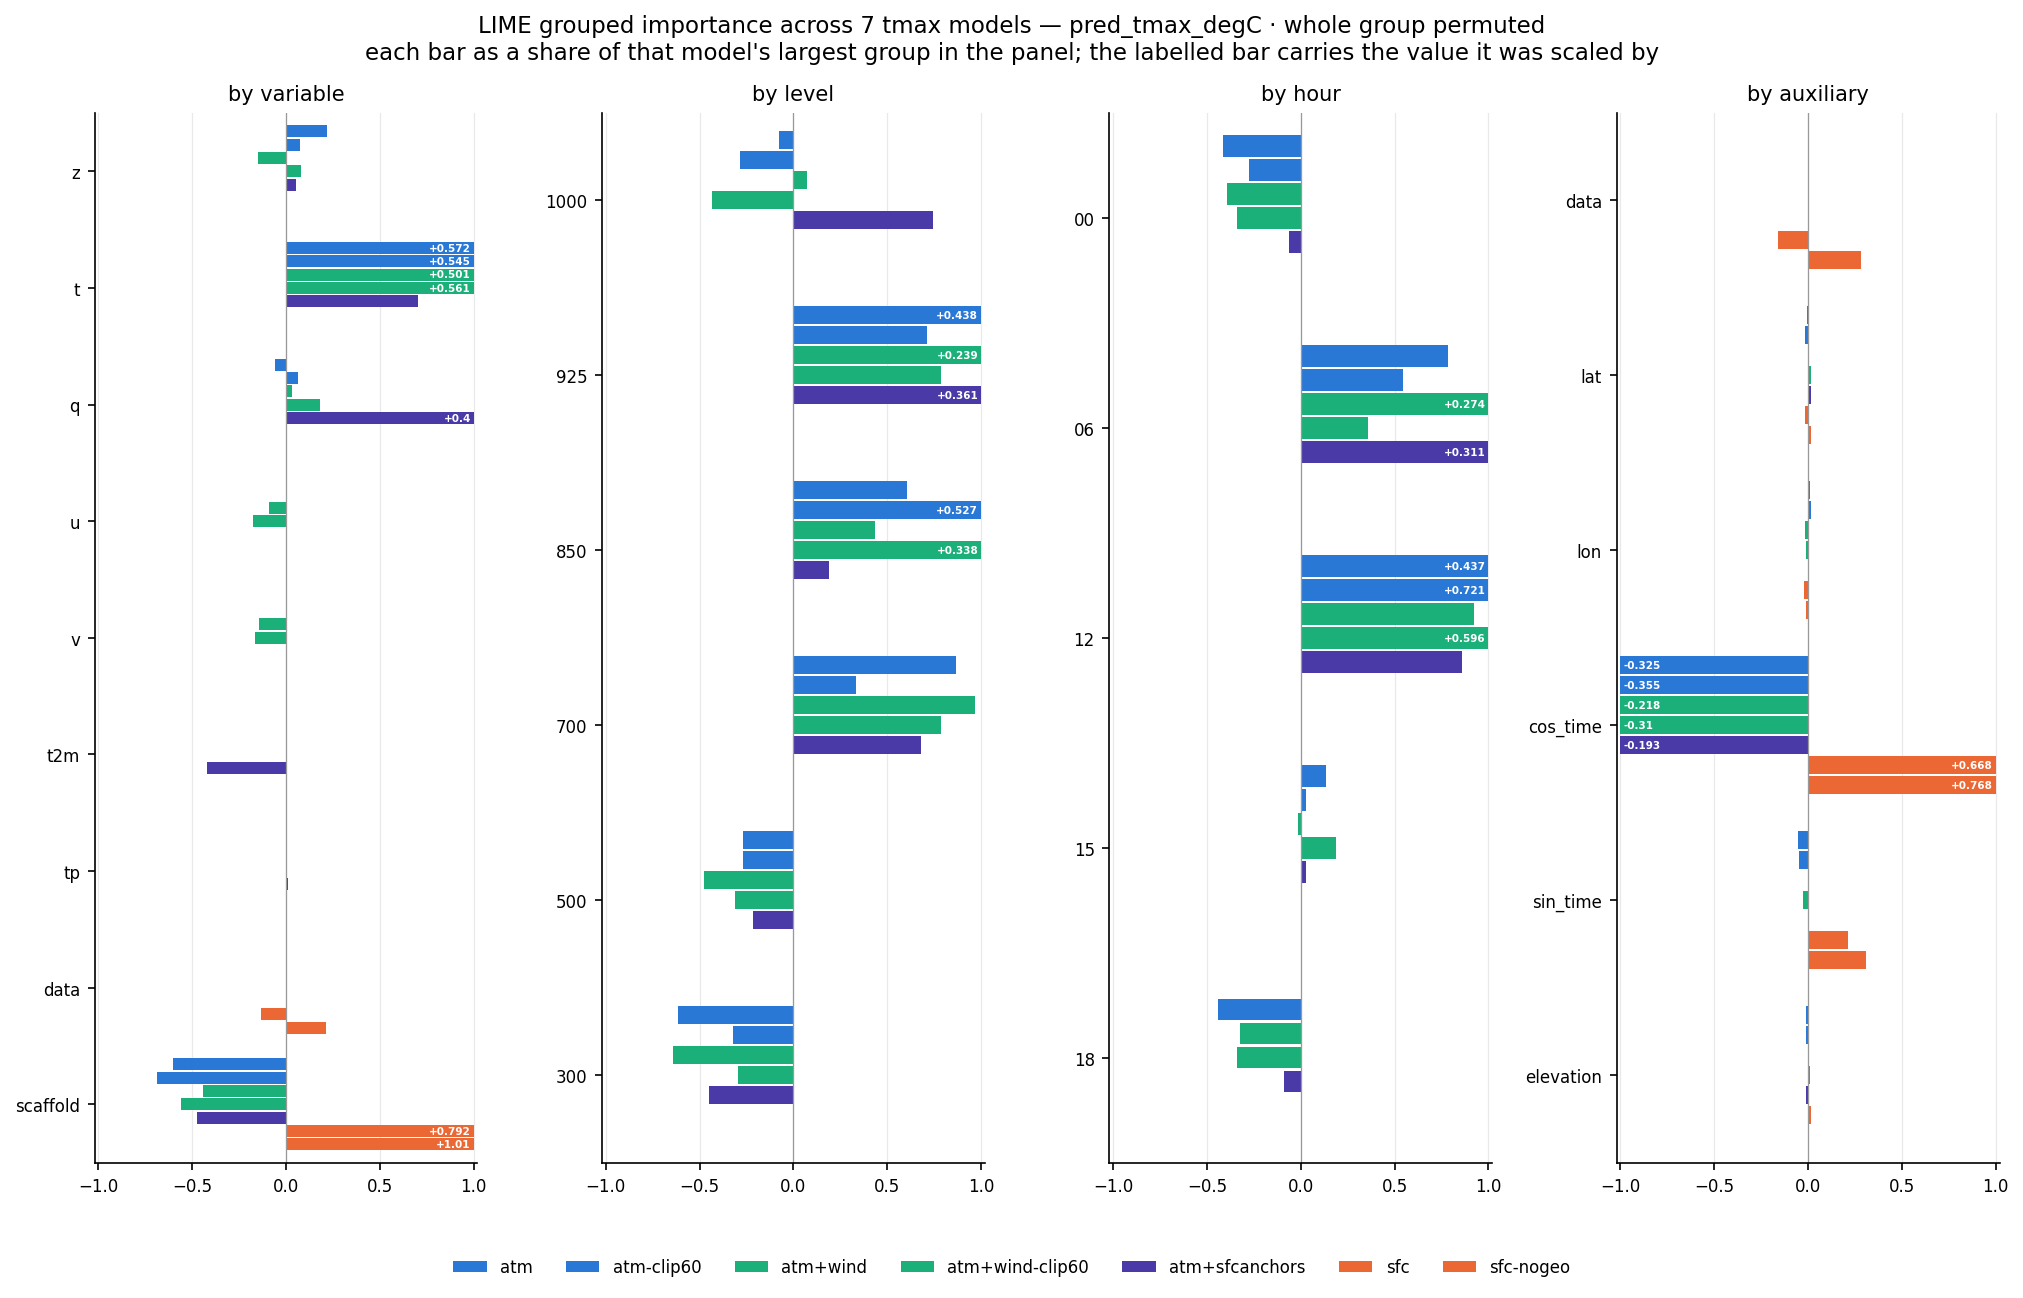
\includegraphics[width=\textwidth]{images/results/tmax__fi_group_importance_lime_2024__tmax_model_comparison__ALL.png}
\caption[Grouped LIME feature importance across all temperature models]{Grouped LIME feature
importance of all seven temperature configurations, normalised as in
\fref{fig:app-fi-all-tmax-pfi}. LIME reports a
signed effect on the spatial-mean prediction, so a bar may point either way and a negative one is a
direction rather than an absence of importance (\sref{subsec:app-fi-lime}).}
\label{fig:app-fi-all-tmax-lime}
\end{figure}

\begin{figure}[h]
\centering
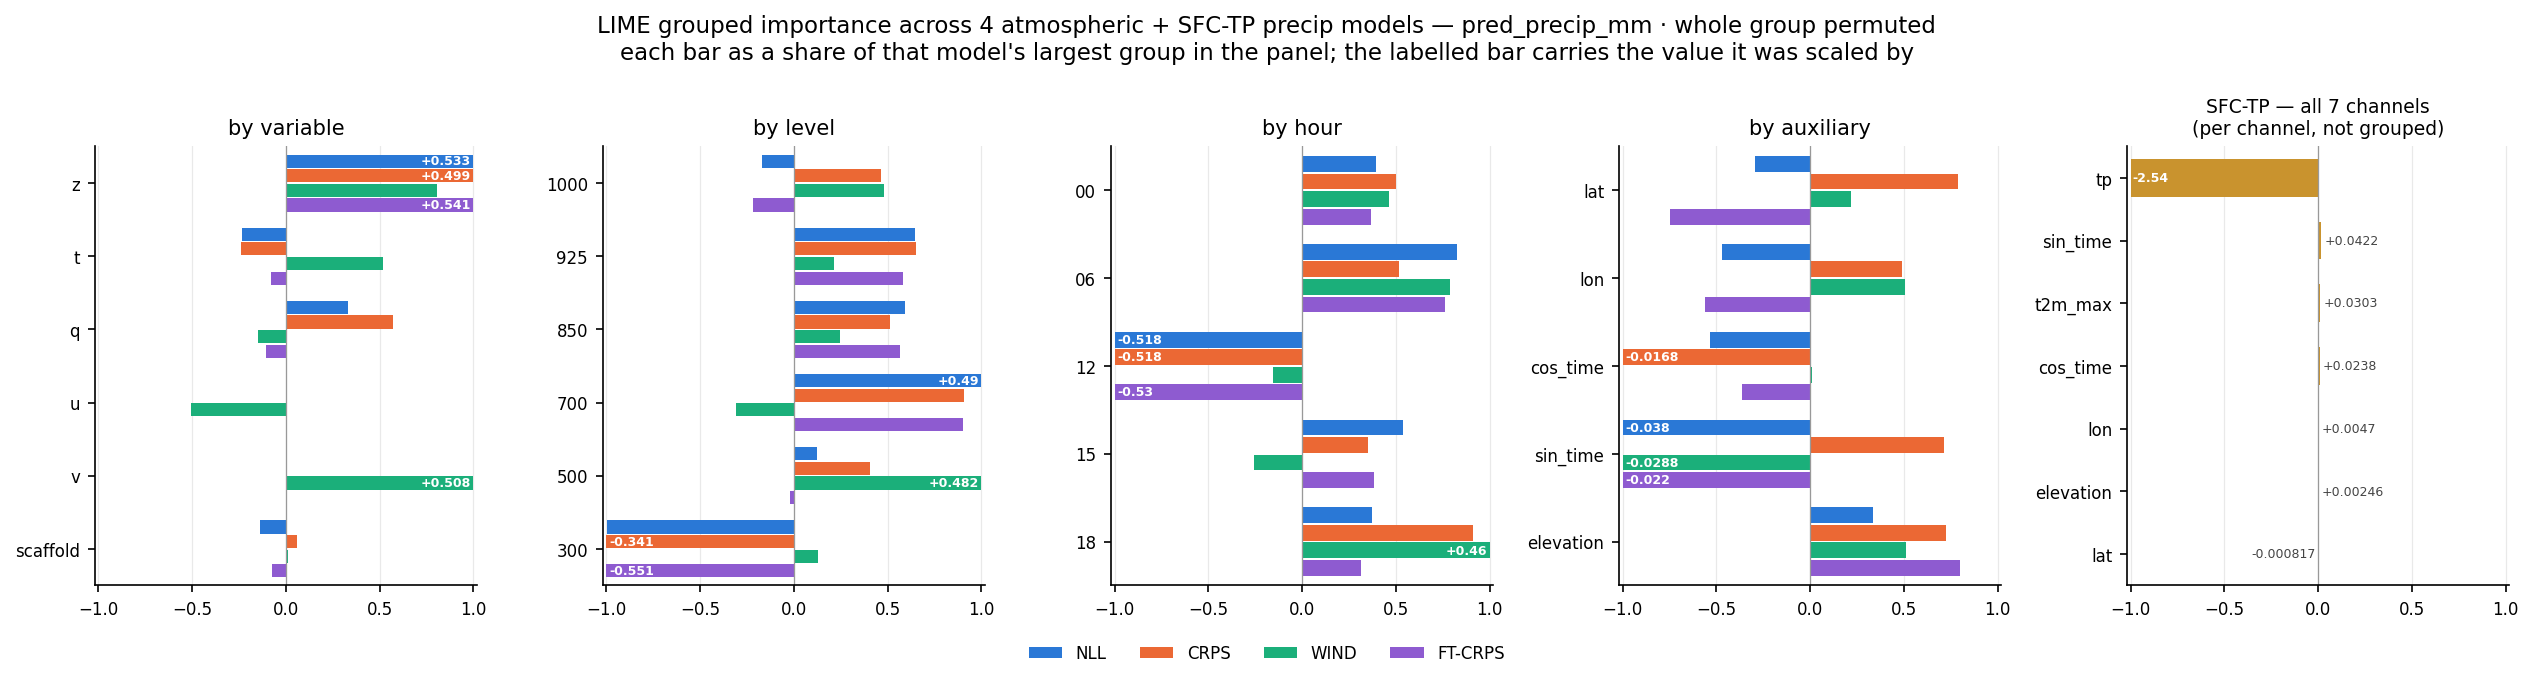
\includegraphics[width=\textwidth]{images/results/precip__fi_group_importance_lime_2024__precip_processing_comparison__ALL.png}
\caption[Grouped LIME feature importance across all precipitation models]{Grouped LIME feature
importance of all five precipitation configurations, normalised as in
\fref{fig:app-fi-all-tmax-pfi}. The permutation
counterpart is \fref{fig:single-precip-fi} in the main text. The disagreement between the two
methods on precipitation is the subject of \sref{subsec:app-fi-lime}.}
\label{fig:app-fi-all-precip-lime}
\end{figure}

\FloatBarrier
\subsection{Limitations of the Permutation Estimator}\label{subsec:app-fi-limits}

Four limitations bound what the importances reported in this work can support.
\begin{itemize}
\item \emph{Static channels are invisible.} Permuting along the day axis leaves a time-invariant
channel unchanged, so latitude, longitude and the coarse elevation score exactly zero by
construction. This is a property of the estimator, not a statement about the model, whose terrain
dependence is carried by the elevation MLP of \sref{subsec:meth-elev-mlp}.
\item \emph{Permutation forces extrapolation.} Pairing a January field with a July target day never
occurs in nature, so part of what is measured is a model queried outside its training
distribution~\cite{hooker2021unrestricted}. Grouping reduces this; only retraining would remove it.
\item \emph{The result describes this model, not the atmosphere.} A low importance means the fitted
model does not depend on that channel, not that the predictor is uninformative.
\item \emph{A shared scale is not a shared verdict.} Importances from different runs can be placed
on one axis, but a model spreading its reliance thinly is not for that reason worse than one leaning
on a few channels.
\end{itemize}

\subsection{The LIME Cross-Check}\label{subsec:app-fi-lime}

LIME explains one prediction by fitting a simple surrogate in a neighbourhood of
it~\cite{ribeiro2016lime}. The neighbourhood used here is built from the presence or absence of
input channels. For a chosen day a thousand binary masks are drawn over the channels; a masked
channel is replaced by its temporal-mean field, so it loses that day's anomaly while keeping its
spatial climatology and the field stays plausible. Each masked context is passed through the
five-fold ensemble and reduced to its spatial-mean prediction, giving one number per mask, and a
weighted ridge regression of that number on the masks returns one signed coefficient per channel,
with masks closer to the unmasked input weighted more heavily. A group coefficient is the sum over
the group's channels. Four days spread through the scored year are explained this way; the bars are
their mean and the error bars their spread.

It is kept as a cross-check rather than as evidence, and the figures above show why. The
coefficients are signed, so they mix a channel's importance with the direction in which that day's
anomaly happened to push the prediction, which is how the surface model's one informative channel
acquires a large negative value. The spread across the four days exceeds the effect for most groups,
so four days cannot support a statement about a model. The spatial field is averaged away before the
surrogate is fitted, and a downscaling model exists to produce spatial structure, so a channel that
redistributes precipitation without changing the domain total is invisible to this target.
Permutation importance has no such bottleneck, because its metric is accumulated over every target
point. And the observations never enter, so LIME measures how strongly the prediction responds to a
channel rather than whether the channel makes the prediction better.

Where the two methods agree, which for temperature is the level of the variable families and the
leading hour, the agreement is worth having: they share nothing beyond the trained model, having a
different perturbation, a different target and a different estimator. Where they disagree, as they
do for precipitation, the permutation result is the one carried forward.

\begin{figure}[H]
\centering
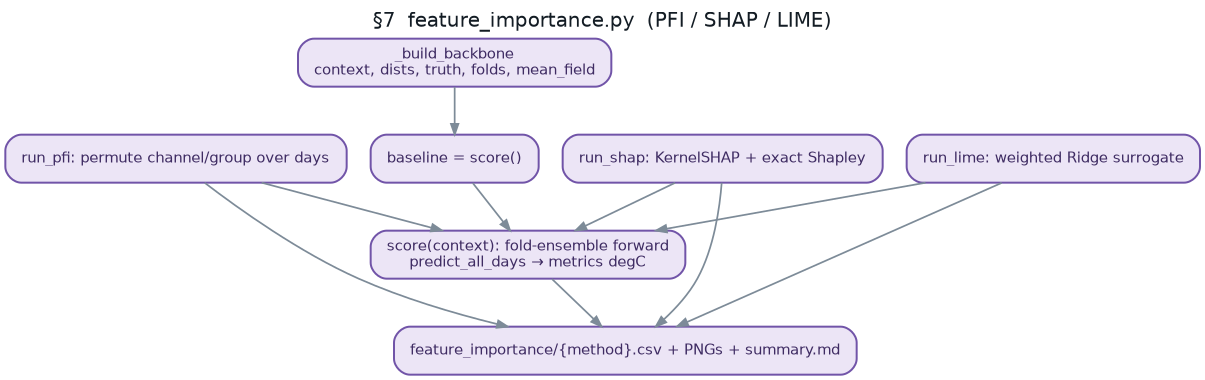
\includegraphics[width=\textwidth]{images/s7_feature_importance.png}
\caption[The feature-importance implementation]{Structure of the feature-importance implementation.
The three methods differ only in the perturbation they apply; all of them score through the same
fold-ensemble forward pass, so the model is treated as a black box throughout.}
\label{fig:app-fi-pipeline}
\end{figure}

\FloatBarrier
\section{Training Curves of the Precipitation Runs}\label{sec:app-precip-training}

The five runs of \tref{tab:single-precip-variants} minimise two different objectives, so the loss
each one descends is not the same quantity: three runs minimise the Bernoulli--Gamma likelihood of
\eref{eq:bg-ll}, \texttt{precip-CRPS} the sampled CRPS of \eref{eq:crps}, and
\texttt{precip-FT-CRPS} the second after converging on the first. The left panel of
\fref{fig:app-precip-training} therefore shows convergence only, each run on its own scale, and
nothing in it may be read as a ranking. The right panel is the one common criterion: the held-out
Bernoulli--Gamma CRPS, which every run reports whatever it was trained on, and which the
fine-tuning stops on.

Read on that criterion, \texttt{precip-FT-CRPS} reaches $1.762$ at its fourth fine-tune epoch
against $1.789$ at epoch $26$ for \texttt{precip-NLL} and $1.832$ at epoch $29$ for
\texttt{precip-CRPS}. A ten-epoch fine-tune budget from a converged likelihood model, ended by early stopping after
four to eight epochs, recovers more of the CRPS than thirty epochs of training on the CRPS from
scratch, which is the evidence behind the fine-tuned
variant being a third run rather than a variation of the second (\sref{objective}). Everything beyond convergence (accuracy,
occurrence, intensity and skill) is a result and is reported in
\sref{subsec:single-precip-headline}, not read off these curves.

\begin{figure}[H]
\centering
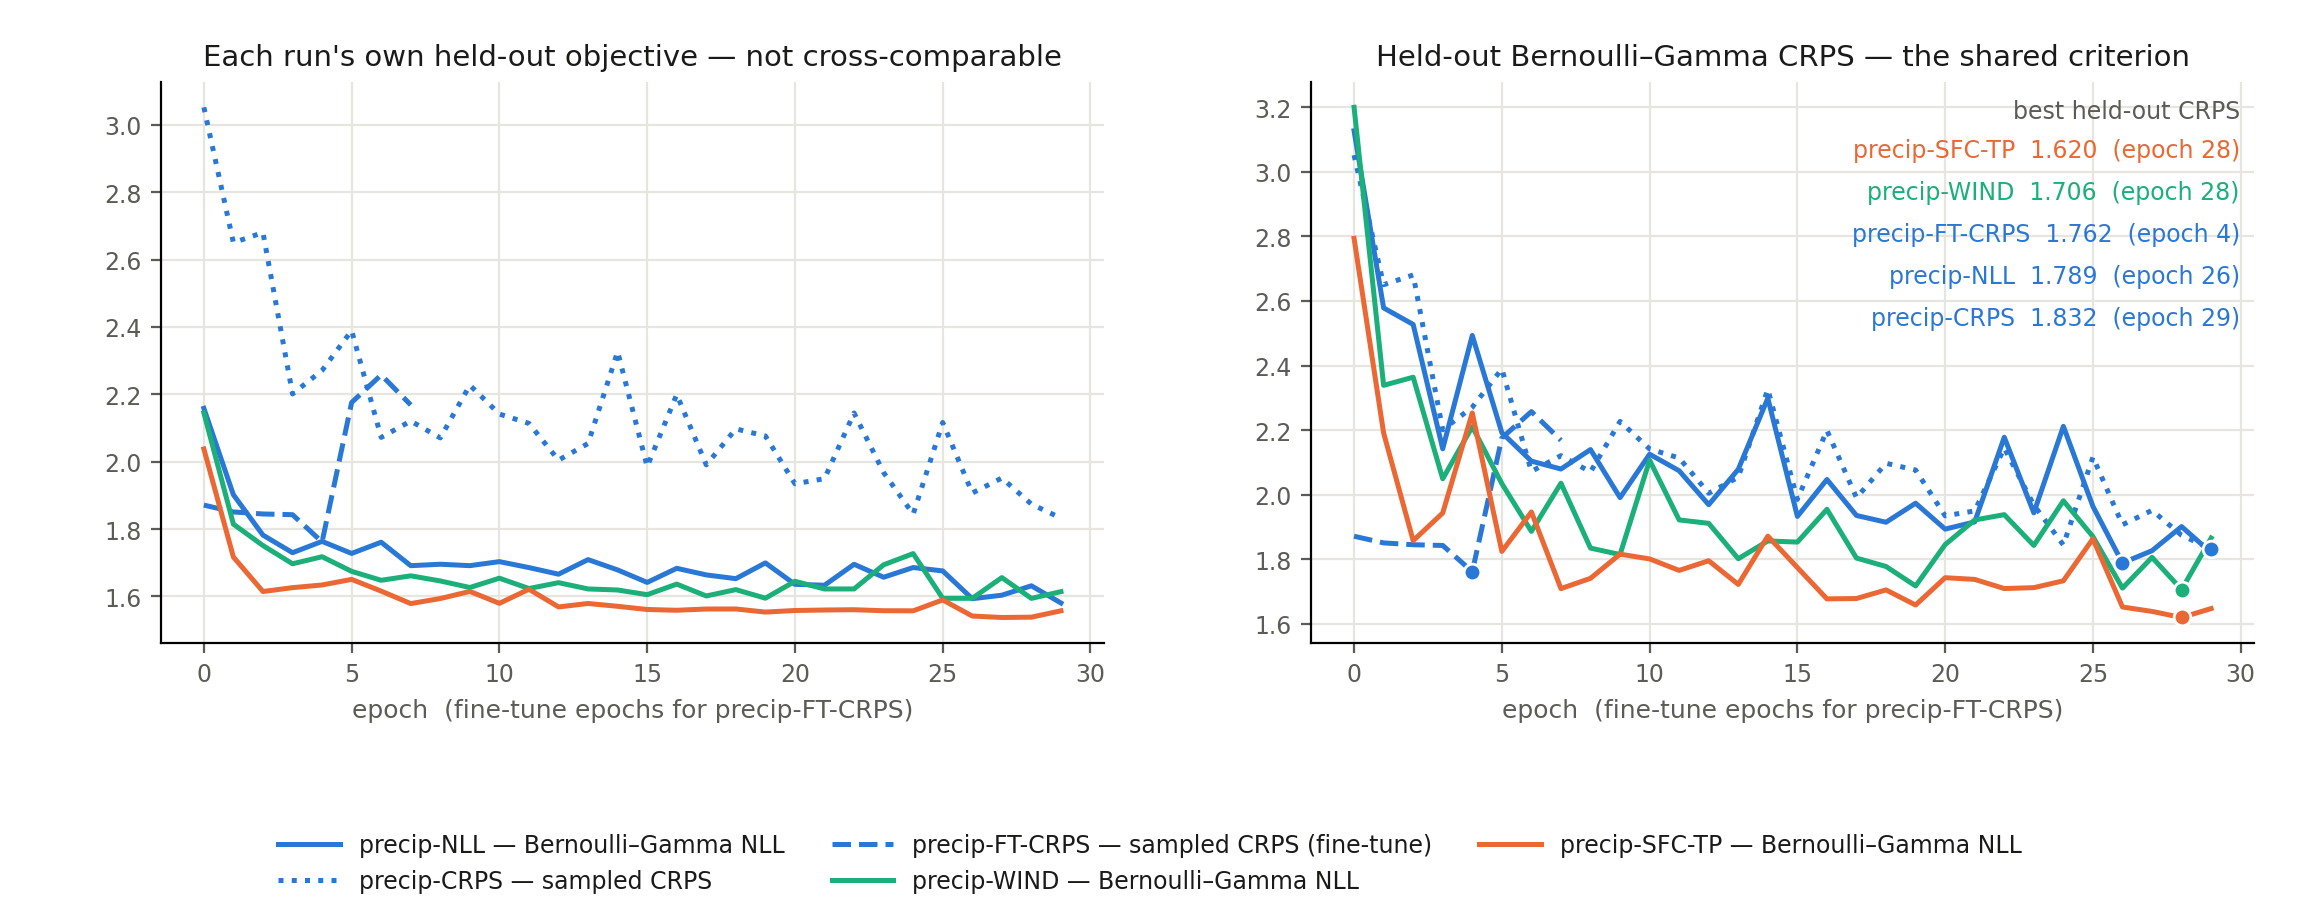
\includegraphics[width=\textwidth]{images/precip_training_curves.png}
\caption[Training curves of the precipitation runs]{Fold-averaged held-out training curves of the
five precipitation runs, on the colour and line-style conventions of
\fref{fig:single-precip-slope}. Left: each run's own objective, which for the two CRPS-trained runs
is the sampled CRPS and for the other three the Bernoulli--Gamma likelihood; the curves converge
but are not comparable to each other. Right: the held-out Bernoulli--Gamma CRPS, the single score
every run shares, with the best epoch marked on each curve. \texttt{precip-FT-CRPS} contributes only
its fine-tune epochs (a ten-epoch budget ended by early stopping), which begin from the converged \texttt{precip-NLL} model, so its epoch
axis counts epochs after the warm start and is not comparable to the from-scratch runs.}
\label{fig:app-precip-training}
\end{figure}

\FloatBarrier
\section{Spatial Intensity Categories for the Remaining Precipitation Runs}\label{sec:app-precip-category-spatial}

\fref{fig:single-precip-spatial-categories} compares \texttt{precip-FT-CRPS} and
\texttt{precip-SFC-TP}, the two runs selected in \sref{subsec:single-precip-selection}. The three
remaining runs are reproduced here on the same five intensity categories, each against the observed
field and the bilinear ERA5-Land reference, with its own Brier skill. Unlike the main-text figure,
these are the per-run renderings, so the frequency colour scale is chosen per figure rather than
shared across runs: read them for pattern and for the skill columns, not for colour-matched
comparison between runs.

\begin{figure}[H]
\centering
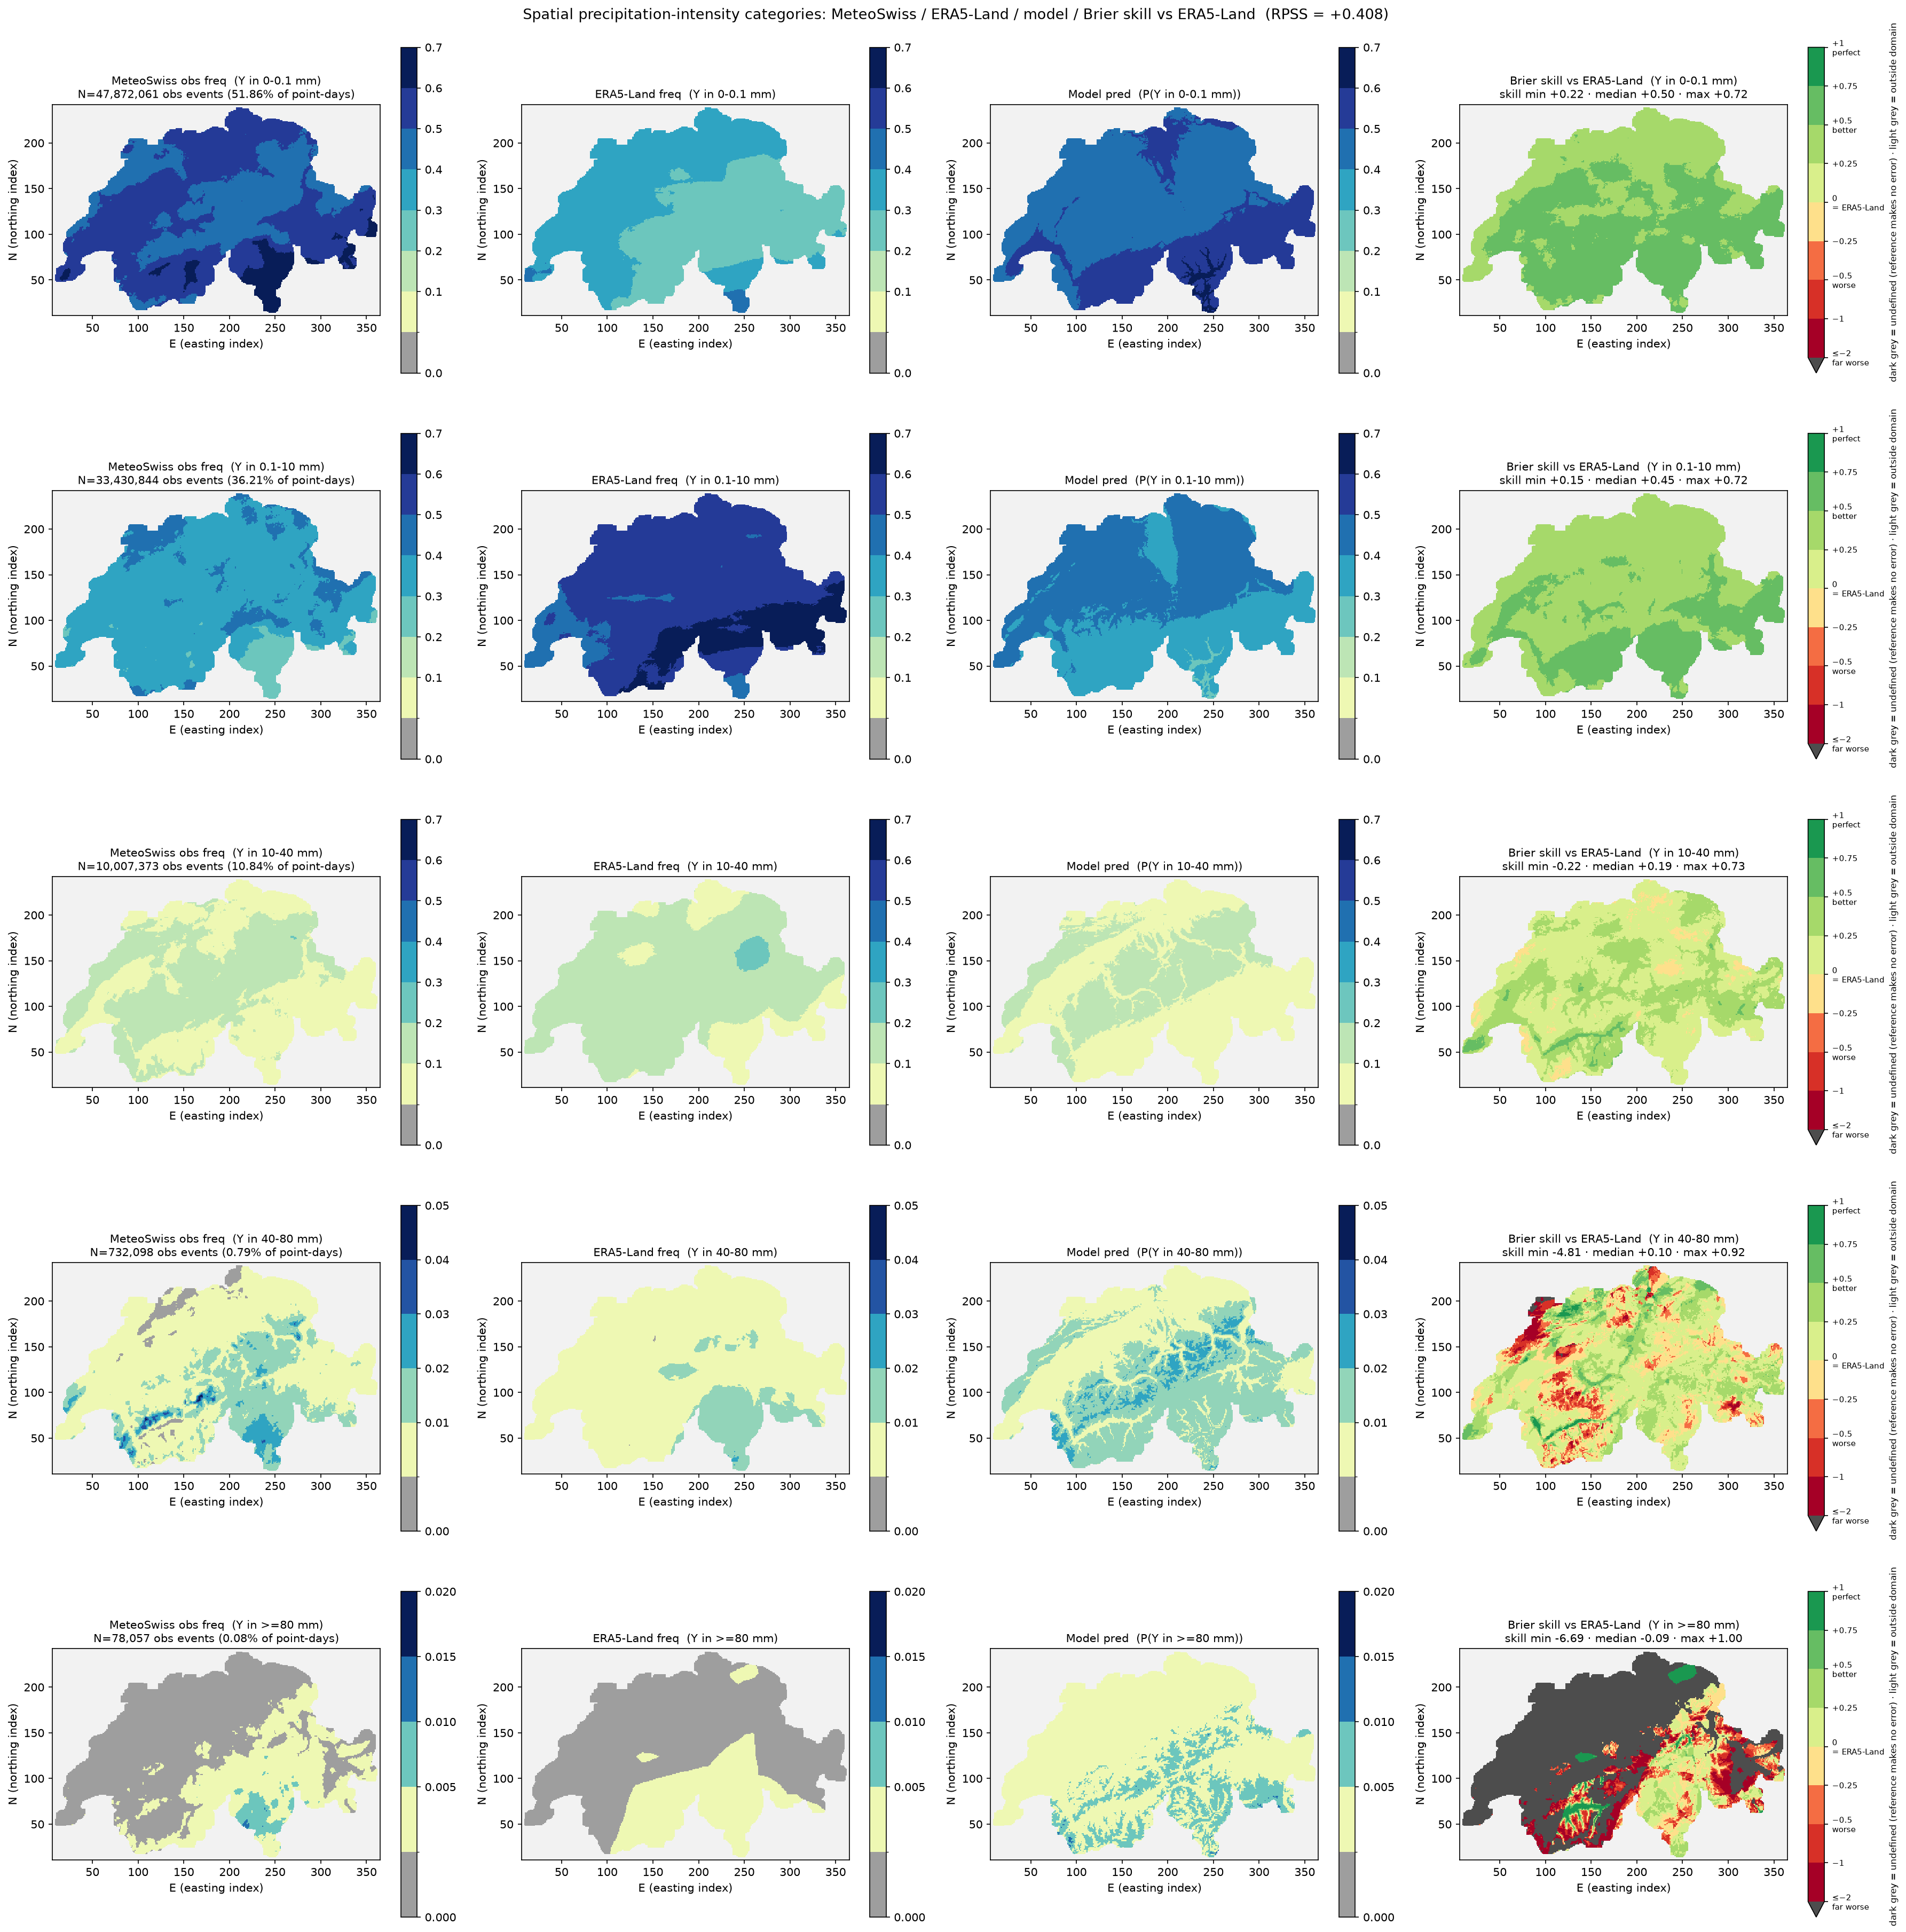
\includegraphics[width=0.92\textwidth]{images/results/precip__precip_category_spatial__eval_cv__clean_solo_precip.png}
\caption[Spatial intensity categories, \texttt{precip-NLL}]{\texttt{precip-NLL} on the CV holdout.
This is the run the naive reference beats on the tail (\sref{subsec:single-precip-headline}), and
the $\geq 80\,\mathrm{mm}$ skill column is correspondingly the weakest of the five.}
\label{fig:app-precip-catspatial-nll}
\end{figure}

\begin{figure}[H]
\centering
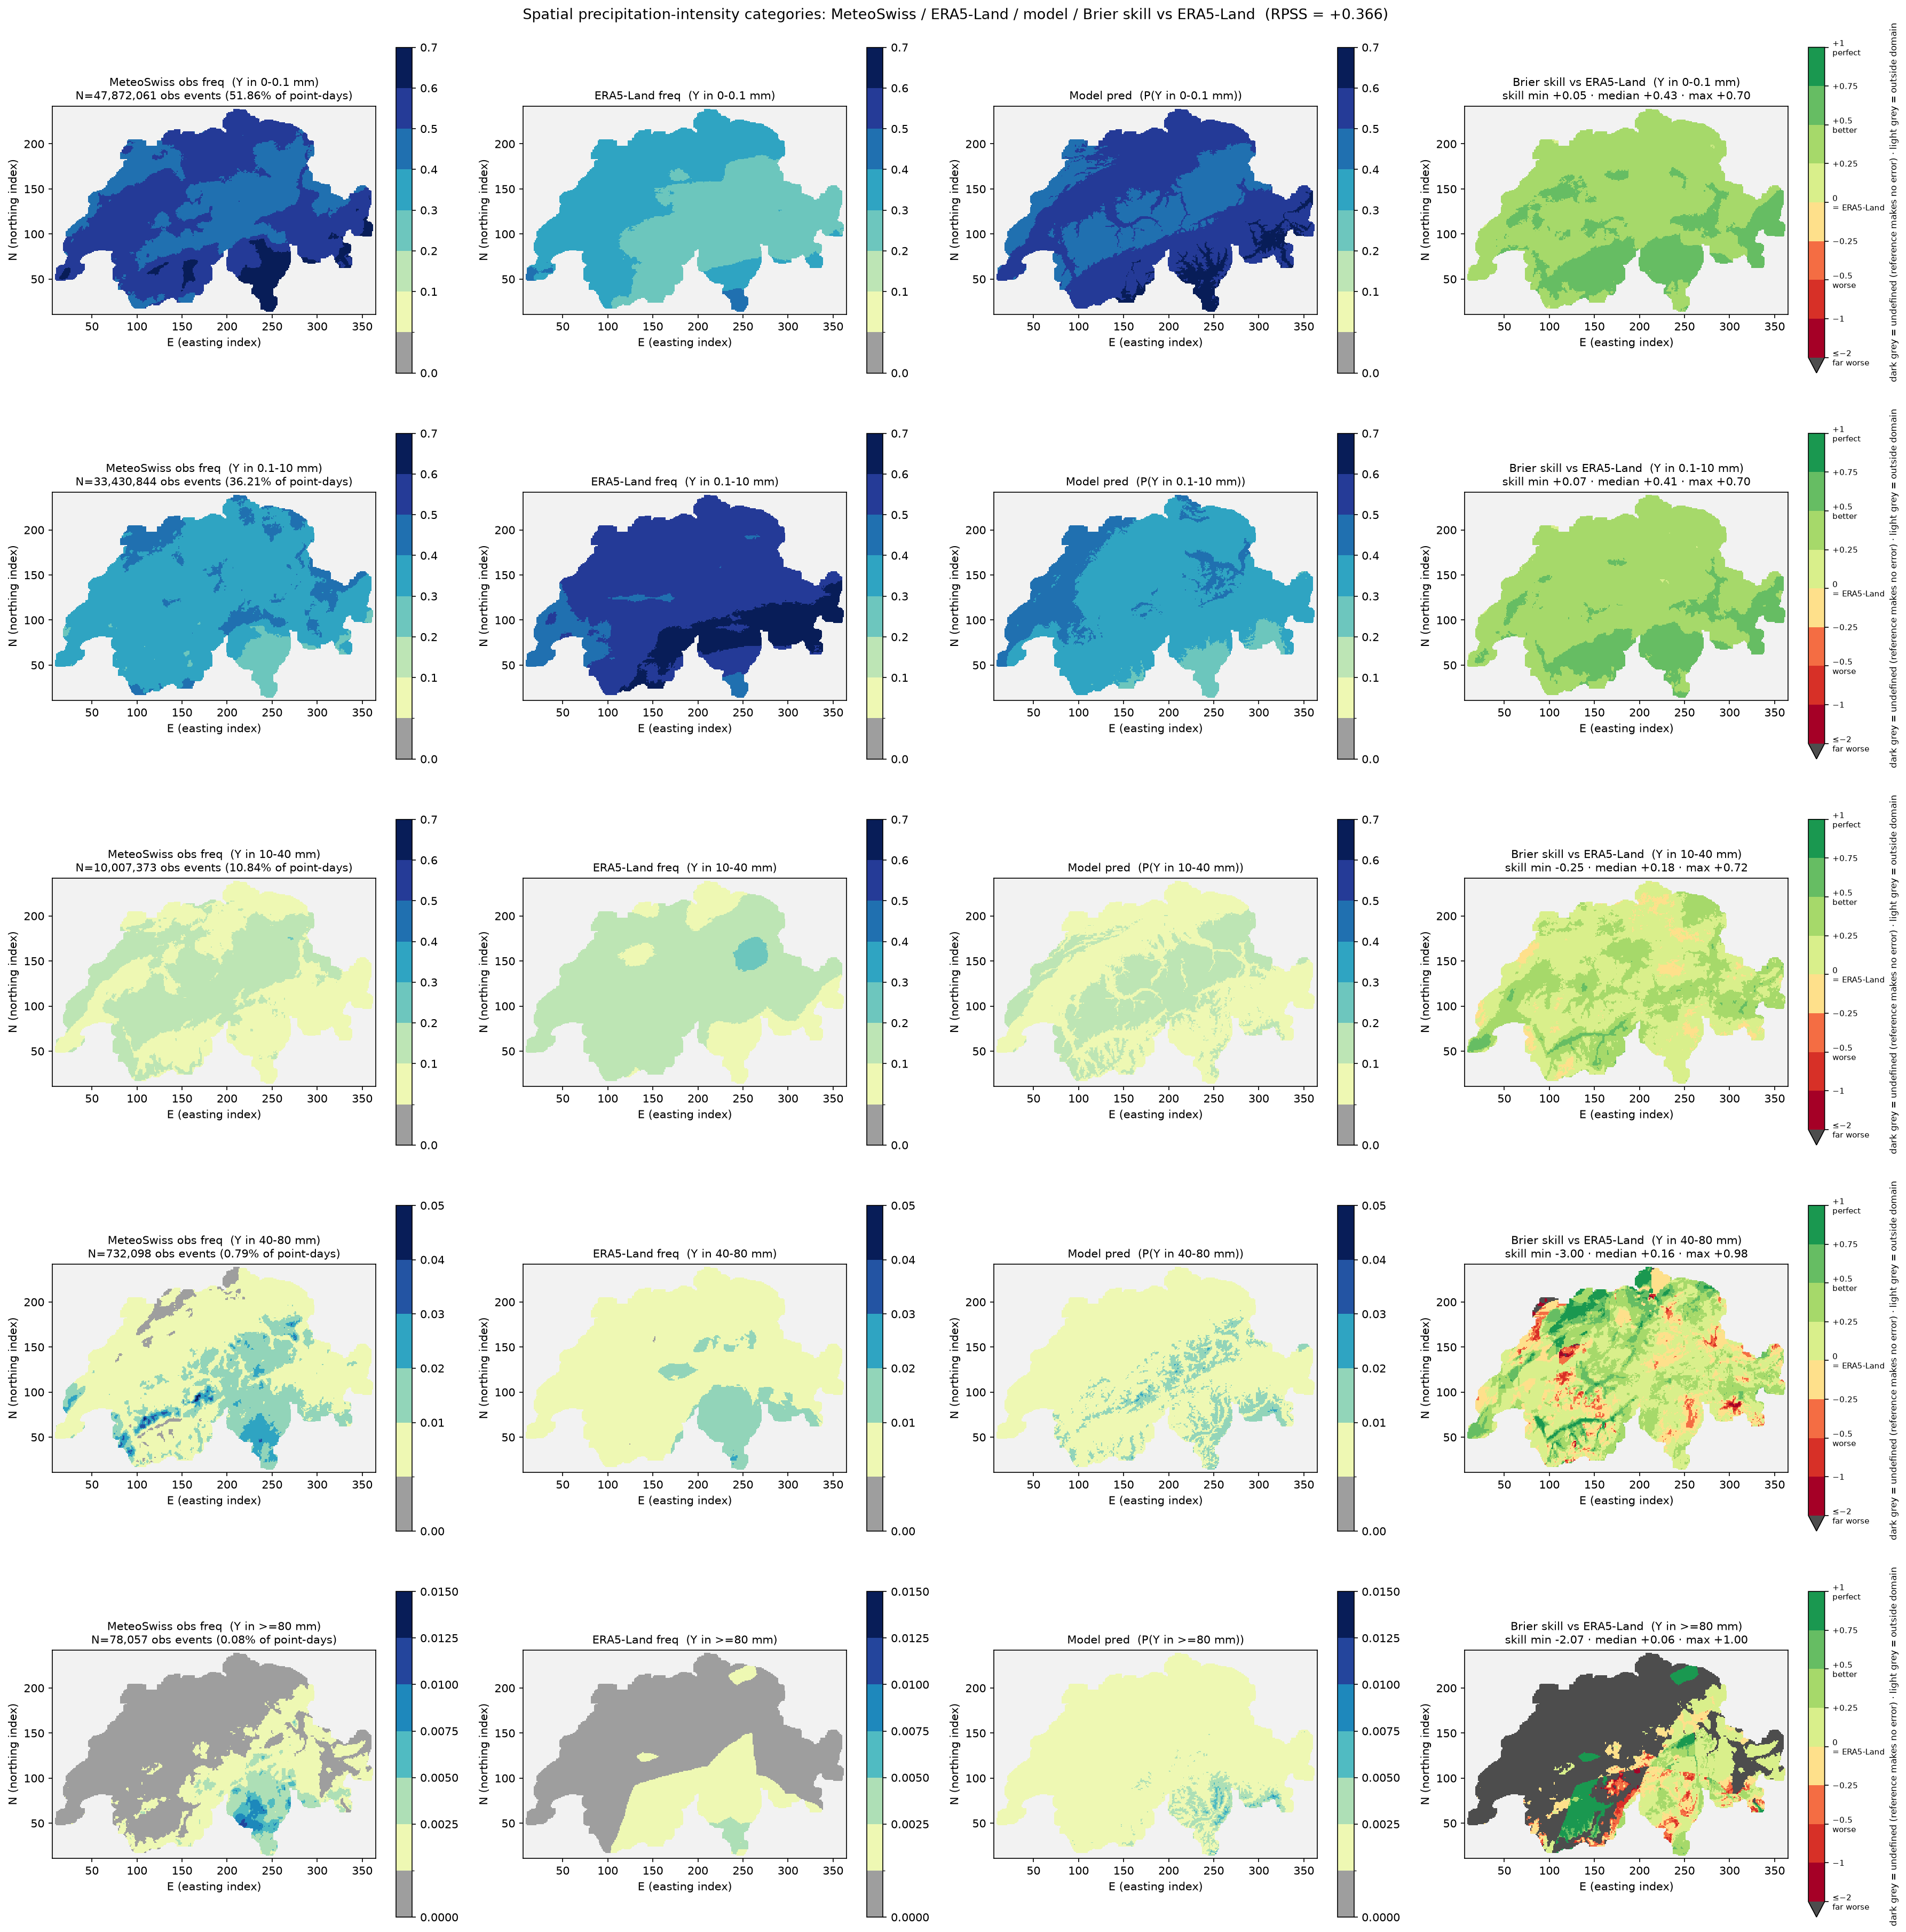
\includegraphics[width=0.92\textwidth]{images/results/precip__precip_category_spatial__eval_cv__clean_solo_precip_crps.png}
\caption[Spatial intensity categories, \texttt{precip-CRPS}]{\texttt{precip-CRPS} on the CV
holdout. The driest of the objectives and the best of the five in the heaviest category on this
regime, bought by being the weakest of the five in the two categories that hold most of the days
(\sref{subsec:single-precip-categories}).}
\label{fig:app-precip-catspatial-crps}
\end{figure}

\begin{figure}[H]
\centering
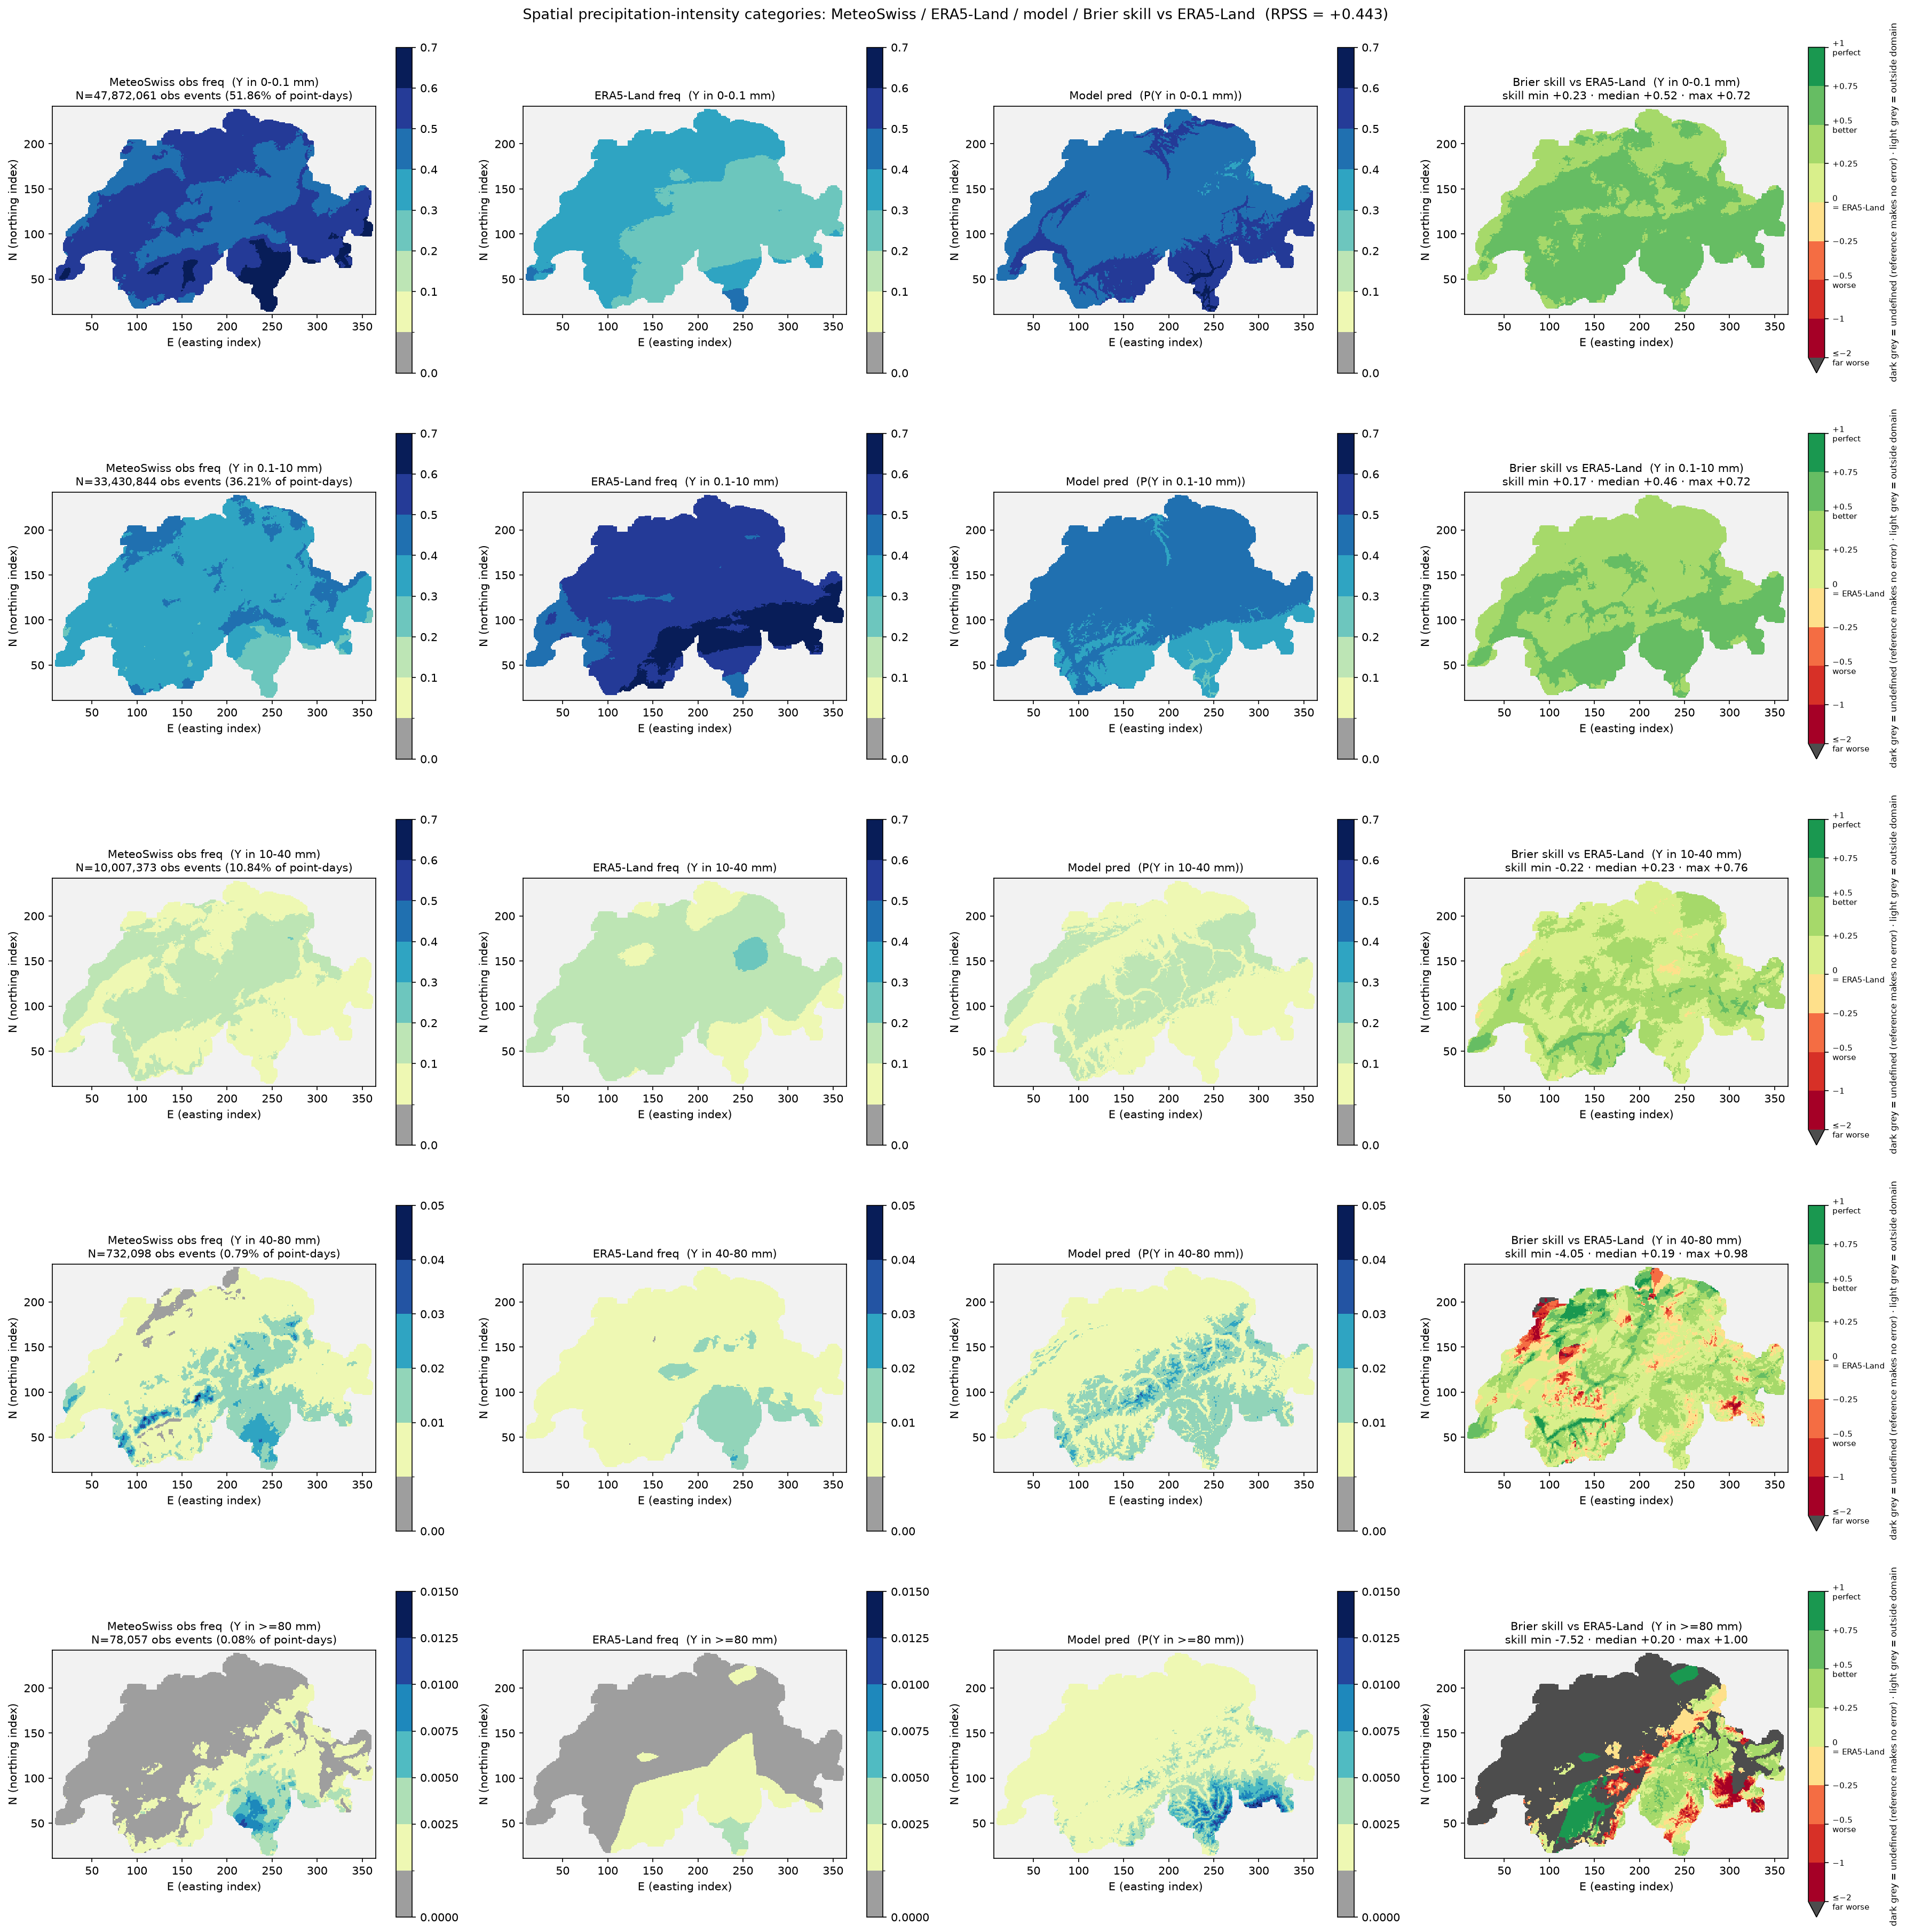
\includegraphics[width=0.92\textwidth]{images/results/precip__precip_category_spatial__eval_cv__clean_solo_precip_wind.png}
\caption[Spatial intensity categories, \texttt{precip-WIND}]{\texttt{precip-WIND} on the CV
holdout, the strongest of the four atmospheric runs on both pooled skill scores
(\tref{tab:single-precip-selection}). Its lead is spread evenly over the first three categories
rather than concentrated anywhere, which is why it does not show as a distinct spatial pattern.}
\label{fig:app-precip-catspatial-wind}
\end{figure}

\section{Station Verification Details}\label{sec:app-stations}

This section carries the data statement behind \cref{ch:stations}: how the three station sets were
selected and checked. A station enters its set if it reports on at least $95\,\%$ of the days in 2020--2024, and is scored
only where enough valid days remain ($10$ for temperature, $30$ for the per-gauge precipitation
scores). The SMN metadata lists $158$ stations, of which $8$ deliver no data in the study window; $149$
report temperature and $139$ operate a rain gauge. The coverage cut removes two temperature
series and no gauge, leaving the $147$ temperature stations and $139$ gauges of
\tref{tab:stations-sets}. The gauge observable is the $06$--$06\,\mathrm{UTC}$ daily
total, the accumulation window RhiresD itself uses \cite{meteoswiss_rhiresd_doc}. The SMN series are operational rather than
homogenised; at the $28$ sites present in both temperature sets, the operational and the homogenised
NBCN series give per-station MAEs identical to a median of $0.00\,^{\circ}\mathrm{C}$ (maximum
difference $0.08\,^{\circ}\mathrm{C}$), so the distinction carries no weight over this span.
